\documentclass[twoside,AutoFakeBold=true]{ZJUthesisv2}
% 该文档中首字符为“%”的均为注释行,不会在论文中出现
% 论文默认为双面模式,需单面模式请将第一行换为如下所示:
% \documentclass[oneside]{ZJUthesis}
% \documentclass[twoside]{ZJUthesis}

% 取消目录中链接的颜色,方便打印
% 如需颜色,请将“false”改为“true”
%\usepackage{hyperref}
\hypersetup{colorlinks=false}

% 这里几行代码使得目录中的“第几章” 和后面的章节名称不致发生重叠
\makeatletter
\renewcommand{\numberline}[1]{%
\settowidth\@tempdimb{#1\hspace{0.5em}}%
\ifdim\@tempdima<\@tempdimb%
  \@tempdima=\@tempdimb%
\fi%
\hb@xt@\@tempdima{\@cftbsnum #1\@cftasnum\hfil}\@cftasnumb}
\makeatother

%\usepackage[sectionbib]{chapterbib}

% \makeatletter
% \def\@chapter[#1]#2{\ifnum \c@secnumdepth >\m@ne
%   \if@mainmatter
%     \refstepcounter{chapter}%
%     \typeout{\@chapapp\space\thechapter.}%
%     \addcontentsline{toc}{chapter}%
%     {\protect\numberline{第 \chaptername 章}\hspace{1em}#1}
% %    {\protect\numberline{\chaptername}\hspace{4em}#1}
%   \else
%     \addcontentsline{toc}{chapter}{#1}%
%   \fi
%   \else
%   \addcontentsline{toc}{chapter}{#1}%
%   \fi
%   \chaptermark{#1}%
%   \if@twocolumn
%   \@topnewpage[\@makechapterhead{#2}]%
%   \else
%   \@makechapterhead{#2}%
% \@afterheading
% \fi}
% \makeatother

\usepackage{enumitem}

\begin{document}
%%%%%%%%%%%%%%%%%%%%%%%%%%%%%
%% 正文字体设定
%%%%%%%%%%%%%%%%%%%%%%%%%%%%%
\songti

%%%%%%%%%%%%%%%%%%%%%%%%%%%%%
%% 论文封面部分
%%%%%%%%%%%%%%%%%%%%%%%%%%%%%
% 中文封面内容

% 中图分类号
\classification{TP242.6}

% 单位代码
\serialnumber{10335}

% 密级,如需密级则将其前“%”去掉
\SecretLevel{无}

% 学号
\PersonalID{21532112}

\title{面向工业装配演示编程的}
% 如果标题一行写不下,就写成两行,在下面的命令里写第二行,不需要两行则注释掉
\titletl{物体六维位姿估计与检测}
% \titletl{test}

%英文题目
\Etitle{6D Pose Estimation and Detecting of Objects for}
% 如果一行写不下,同中文题目设定,一行写不下则写两行,不需要就注释掉
\Etitletl{Industrial Programming by Demonstration}

% 作者
\author{陈乙宽}

\degree{硕士}

% 导师
\supervisor{熊\quad 蓉\quad 教\quad 授}

% 合作导师,如果有的话,去掉注释,
%\cpsupervisor{某 \quad某某}

% 专业名称
\major{控制科学与工程}

% 研究方向
\researchdm{机器人}

% 所属学院
\institute{控制科学与工程学院}

%论文提交日期
\submitdate{2015年4月8日}

% 答辨日期
\defenddate{2015年6月12日}
\defenddateE{June 12th, 2015}

% 生成封面
\makeCoverPage

%%%%%%%%%%%%%%%%%%%%%%%%%%%%%%
%% 中文题名页内容
%%%%%%%%%%%%%%%%%%%%%%%%%%%%%%
% 论文评阅人信息 注意两字名与三字名,两字职称与三字职称的写法,便于对齐
% 多余的名额直接注释掉即可,比如三个评阅人,把评阅人D,E注释掉即可
\reviewersA{丘处机\hspace{1.5em}真人\hspace{1.5em}登州滨都宫\hspace{1em}}
\reviewersB{葛\quad 洪\hspace{1.5em}方士\hspace{1.5em}罗浮山道观\hspace{1em}}
\reviewersC{寇谦之\hspace{1.5em}天师\hspace{1.5em}嵩山中岳道场}
\reviewersD{张三丰\hspace{1.5em}真君\hspace{1.5em}武当玉虚宫\hspace{1em}}
\reviewersE{孙玄清\hspace{1.5em}真人\hspace{1.5em}崂山明霞洞\hspace{1em}}

% 答辩委员会信息,如果某一个单位比较长,
% 请在其它较短后面补上{hspace{Xem}},X是比最长的单位名少几个字
% 如果实际人数少于6人,多余的注释掉即可
\chairman{唐三藏\hspace{1.5em}功佛\hspace{1.5em}洛阳大慈恩寺}
\commissionerA{惠\quad 能\hspace{1.5em}方丈\hspace{1.5em}曹溪宝林寺\hspace{1em}}
\commissionerB{智\quad 顗\hspace{1.5em}方丈\hspace{1.5em}天台山国清寺}
\commissionerC{法\quad 藏\quad 大和尚\quad 洛阳佛授记寺}
\commissionerD{道\quad 济\hspace{1.5em}和尚\hspace{1.5em}临安灵隐寺\hspace{1em}}
\commissionerE{降\quad 龙\hspace{1.5em}尊者\hspace{1.5em}天竺大雷音寺}

% 生成中文题名页
\maketitle


%%%%%%%%%%%%%%%%%%%%%%%%%%%%%%
%% 英文封面内容,硕士论文可不要此页
%%%%%%%%%%%%%%%%%%%%%%%%%%%%%%
%英文题目
\Etitle{6D Pose Estimation and Detecting of Objects for}
% 如果一行写不下,同中文题目设定,一行写不下则写两行,不需要就注释掉
\Etitletl{Industrial Programming by Demonstration}
% % 英文题名
% \englishtitle{HVlab~\LaTeX~Fast Guide}
% % 如果题名一行写不下,就写到第二行,不需要则将其注释掉
% \englishtitletl{The Second Edition}

% 评阅人信息,名字,职称,单位尽量用简写,否则会写不下
\EreviewersA{Name\hspace{1.5em}Professional Title\hspace{1.5em}Organization}
\EreviewersB{Name\hspace{1.5em}Professional Title\hspace{1.5em}Organization}
\EreviewersC{Name\hspace{1.5em}Professional Title\hspace{1.5em}Organization}
\EreviewersD{Name\hspace{1.5em}Professional Title\hspace{1.5em}Organization}
\EreviewersE{Name\hspace{1.5em}Professional Title\hspace{1.5em}Organization}

% 答辩委员会信息,同样尽量用简写,否则会写不下
\Echairman{Name\hspace{1.5em}Professional Title\hspace{1.5em}Organization}
\EcommissionerA{Name\hspace{1.5em}Professional Title\hspace{1.5em}Organization}
\EcommissionerB{Name\hspace{1.5em}Professional Title\hspace{1.5em}Organization}
\EcommissionerC{Name\hspace{1.5em}Professional Title\hspace{1.5em}Organization}
\EcommissionerD{Name\hspace{1.5em}Professional Title\hspace{1.5em}Organization}
\EcommissionerE{Name\hspace{1.5em}Professional Title\hspace{1.5em}Organization}

% 生成英文封面
\makeenglishtitle


%%%%%%%%%%%%%%%%%%%%%%%%%%%%%%
%% 原创声明与版权协议页
%%%%%%%%%%%%%%%%%%%%%%%%%%%%%%

\SignautreDateA{}{}{}
\SignautreDateB{}{}{}
\SignautreDateC{}{}{}
% 生成原创声明与版权协议页
\makeOSandCPRTpage


%%%%%%%%%%%%%%%%%%%%%%%%%%%%%%
%% 论文部分开始
%%%%%%%%%%%%%%%%%%%%%%%%%%%%%%
\ZJUfrontmatter

%%%%%%%%%%%%%%%%%%%%%%%%%%%%%%
%% 勘误页,一般没有
%%%%%%%%%%%%%%%%%%%%%%%%%%%%%%
%\begin{corrigenda}
这是一个勘误\index{勘误}章节,一般情况下是没有的。
\end{corrigenda}


%%%%%%%%%%%%%%%%%%%%%%%%%%%%%%
%% 致谢页
%%%%%%%%%%%%%%%%%%%%%%%%%%%%%%
\begin{thanks}
在我写这个文档的过程中,得到了网络上很多网贴的帮助,在此感谢baidu,Google,感谢
~CTeX 社区http://www.ctex.org,\LaTeX{}学习园地:http://blog.sina.com.cn/wangzhaoli11,
中科大~CTAN~镜像http://mirrors.ustc.edu.cn/CTAN/,水木社区\TeX{}版等网站、论坛,
其他一些较小的个人网站,论坛不再一一点名,在此一并感谢。
感谢浙江大学数学系提供的原始模版,感谢88\TeX{}版。
\end{thanks}


%%%%%%%%%%%%%%%%%%%%%%%%%%%%%%
%% 序言页
%%%%%%%%%%%%%%%%%%%%%%%%%%%%%%
% \begin{preface}
	
一晃又是快两年过去了,在使用中,我又对这个模版的部分内容进行了一定的微调,主要体现在:目录默认为分层结构,不再是以前默认是都顶格的结构;对脚注与正文的距离进行了调整,避免出现以前版本中的脚注离底部距离过大的问题;增加了对子图的支持;修正了第四级标题的字体等。整体上与上一版的没有大的区别,只有一些外观上的优化。这一版也基本是这个模版的最终稿了。接下来的部分仍然是以前的序言,仍然跟在下面。
	
上一版发布于2011年10月26日,发布之后的近两年来,陆陆续续收到一些邮件问关于使用中的一些问题,
我也算基本上做到一一解答。
同进也在着手准备根据提到的问题对这一版模版进行一定的修订,增补一些使用中普遍关心的难点问题。
因为事务冗杂缠身,加上关于参考文献格式调整部分的内容一直没有时间看明白,这个事情就一直拖下来了。
直到前一段断断续续看完了参考文献格式整理部分的帮助资料,搞清楚了它的实现思路原理,
才算又着手修订这一版教程。

在这过去的一年多里,接触到了\XeTeX{},对其强大的直接调用系统字体的能力表示赞叹,
于是将这个模版切换到了\XeTeX{}的环境下,将文件代码换成了对多语言兼容更好的UTF-8代码,
但同时保留对GBK码的兼容,具体不同之处会在后面的章节中提到。
因此新的一版分为UTF-8和GBK两个版本进行发布,两个版本使用上只有很细微的区别,
一般使用过程中可以忽略这个差别。

以下是原来的序言,此处照旧附上。


很早就听说过\LaTeX\index{\LaTeX}了,但却一直没有真正学习过,直到今年,需要处理一些大文档,想起了\LaTeX{}。
重新翻出\LaTeX{}的文档,从CCT开始,至于为什么是CCT,
因为Ctex\index{CTeX}提供的那个CTeX FAQ里对中文的第一个例子,就是以CCT
为例写的。
CCT是中科院的张林波研究员写的,帮助文档都是中文,看起来比较容易,但毕竟是好几年前的版本了,
更新也并不是那么及时,而且CCT\index{CCT}早期版本的字体是点阵字体,边缘很粗糙,
虽然不影响打印,但在这个年代还在用着这样的字体,着实不是那么舒服。
我又开始了第二个例子,CJK的尝试,在尝试CJK\index{CJK}的过程中,
无意中看到了CTeX的ctexart,ctexbook和ctexrep这几个基本模版,这才找到CTeX的门,
筒子们不要笑我绕了这么一大圈才摸进了CTeX的门,虽然从开始就使用的是CTeX的发行版。

这里也要说一下,CTeX提供的部分帮助文档内容也比较老了,一些操作现在新的软件虽然仍然兼容,
但已经不是新版软件推荐的做法了,比如,CTeX FAQ里面对于pdf文件的生成,
依然是先由latex.exe生成dvi文件,再由dvi文件生成ps文件,最后再生成pdf文件。
实际上,现在流行的新版\TeX{}类软件都已经将pdfTeX\index{pdfTeX}作为默认引擎,支持直接生成pdf文件,
而且dvi、ps文件的打开速度比pdf反而要慢许多。我使用的是64位系统,CTeX提供的安装包只支持32位系统,
我单独安装的MikTeX\index{MikTeX} x64\index{x64}版使用CTeX模版生成的dvi文件使用dvips\index{dvips}处理时会找不到字体,
因为这个问题,我找了很久,最后的结论是:dvips可以放弃了,直接使用dvipdfm\index{dvipdfm}更合适。

后来几天在\LaTeX{}的实践中看不少相关细节,开始对其模版产生了兴趣,
在88上\TeX{}版把置顶的ZJUthesis下了下来,就是写这个模版的基础,数学系模版。
下下来后发现这个模板给的例子pdf与当前学校使用的2008年论文模版差别老大了,从封面到目录,
章节格式,都是完全不一样,因此,决定着手做一个与学样提供的Word模版比较接近的模版。

在以2006年数学系模版为基础进行新模版编写的过程中,学了不少方法,
也发现老模版不少过时或者不合适的地方。
第一个学到的就是,从模版一开头就发现这个模版是以ctexbook这个模版为基础制作的,
做到模版完成的时候,
发现88的\TeX{}版置顶模版已经更新,我以为我白做了,
下下来一看,原来这个新的模版不是以ctexbook为基础制作的,而是更基础的\LaTeXe\index{\LaTeX}
对比自己基本完工的模版,才发现ctexbook为我省了很多工作量。只是一些修修改改就做到了很接近学校
word模版的效果。
ctexbook的新版已经直接将hyperref包打了进去,2006年数学系模版对hyperref\index{hyperref}的引用判断部分已经明显示过时,在用新版MikTeX运行的时候直接报错了。
在编写封面的时候,发现2006年的模版用了一个五列的表格,可这部分的内容只需要两列就够了,
直到我某天下载了中科院的模版后才明白,2006年版模版是从中科院模版改编而来,
中科院模版在封面上名字等内容的排列方式需要采用五列表格。这一部分,我也将其重新编写。

随着时代的推进,\LaTeX{}的各种功能包日渐丰富,很多过去只能从\LaTeXe{}代码写的功能,
如今可以通过相应的功能包直接实现,在这个模版中,我使用了几个新的功能包,
其中最新的当属刚刚发布的hyperref更新包,增加了hidelinks命令,可以直接将链接的边框去掉,
不用采用将边框颜色设为白色的方式了。

就像\LaTeX{}的版本总是在接近$\pi$的值一样,这份模版并不是完美的,比如对数学系的定理体系支持不足,
留在以后版本再发布或者请有兴趣的爱好者共同修改。编写这一版本的基本目的是没有任何\LaTeX{}基础的同学可以比较轻松地利用它给自己的毕业论文排一个满意的版面,整个模版没有留太多选项,
可供修改的选项只有两个:单面双面的选择和链接的颜色的有无。在模版中,我对绝大多数的语句,
都做了中文注释,解释其作用,方便有兴趣的同学研究,我也是一个初学者,作出的这份模版,
我想,应该是比较适合初学者胃口的。

\end{preface}


%%%%%%%%%%%%%%%%%%%%%%%%%%%%%%
%% 摘要
%%%%%%%%%%%%%%%%%%%%%%%%%%%%%%
\begin{abstract}
% 随着工业机器人应用领域的不断发展,简化机器人编程、降低对专业人才依赖、加快编程速度成为一个重要发展需求,也成为工业机器人领域的重要研究课题之一。演示编程提供了一种新的向机器人传递信息的方式,是简化机器人编程的重要途径。与传统机器人编程方法相比,它可以大大降低行业应用技术人员在机器人使用和编程方面所需的专业性知识要求,对于机器人的推广应用具有重要意义。物体的六维位姿估计是演示编程技术中一个非常重要的环节。通过自动化的视觉系统对工业零件进行位姿估计,可以简化机器人编程中对机器人操作点位的部署过程,从而提高工业生产的效率。但目前没有一套较为实用的物体位姿估计算法,因此本文提出了一套简单易用的物体六维位姿估计算法框架,其核心思想对于演示编程技术的发展具有一定促进意义。本文主要研究内容与成果如下:
随着工业机器人应用领域的不断发展,物体的六维位姿估计是成为当下进一步提高自动化水平的一个重要研究内容。通过自动化的视觉系统对工业零件进行位姿估计,可以简化对机器人操作点位的部署过程,大大解放人力,从而提高工业生产的效率。本文面向目前柔性制造领域中工业零部件存在姿态随机、存在局部遮挡等问题提出了一套简单易用的物体六维位姿估计算法框架,其核心思想是通过仿真环境借助级联回归框架来构建物体位姿估计模型。本文主要研究内容与成果如下:

\begin{itemize}
\item 归纳整理了随机蕨算法应用于回归问题的解决方案,并提出了一种面向大噪声干扰增加掩码机制的改进随机蕨回归算法。随机蕨算法在研究初期被用于解决分类问题,具有比随机森林算法更为优秀的精度以及效率,但缺点在于不能应用于回归问题。本文通过总结前人经验,给出了随机蕨算法应用于回归问题的解决方案。并针对实际问题中很多特征输入存在较大干扰的情况,提出了一套改进的随机蕨算法。经过本文改进后的随机蕨算法可以利用较易获取的特征置信度掩码进行有选择作出修正,使得随机蕨算法在遇到局部大噪声干扰的情况下仍然可以保持较好的回归精准度,提升了鲁棒性。

\item 搭建了一套深度相机仿真环境平台,通过借助OpenGL工具,能够实现在短时间内给出大量带有真值标注的仿真深度图像数据。这些仿真数据可以用于训练对应工业零件的位姿估计模型,从而为物体位姿估计算法开发提供了高效方便的基础环境。该仿真环境能够预先加载工业现场的深度背景信息,同时也可以模拟复杂环境下物体被随机遮挡的情况,使得最后得到的仿真深度图像更为真实以及丰富,从而让位姿估计模型的训练结果与真实数据训练出的模型更为接近。最后还提出了如何对真实深度相机采集到的深度图像中的空洞进行修补的办法,进一步缩小了仿真深度图像与真实深度图像之间差别。

\item 提出了一种像素差特征的图像特征描述方法和采用改进随机蕨回归的物体六维位姿估计算法。首先提出了一种基于深度图像中的像素差特征的全新深度图像特征描述方法。该特征描述方法具有非常高的计算效率,同时具有尺度不变性,能够很好捕捉深度图像中指定位置的物体位姿信息。然后采用有监督学习的特征哈希表达方法,显著提高原始特征的信噪比,使得物体位姿估计模型的训练更加鲁棒。随后借助本文提出的随机蕨回归算法,提出了一套针对物体位姿估计的级联回归算法框架,修正了普通级联回归算法框架中回归目标过于固定的不足。最后还利用改进后的随机蕨回归算法,提出了一种遮挡情况下物体位姿估计算法,以及利用位姿回归所用的特征描述进行物体检测,形成一套完整的从物体定位到物体位姿估计算法框架。
\end{itemize}


\keywords{位姿估计,随机蕨,仿真深度相机,物体检测}
\end{abstract}


%%%%%%%%%%%%%%%%%%%%%%%%%%%%%%
%% 英文摘要
%%%%%%%%%%%%%%%%%%%%%%%%%%%%%%
\begin{englishabstract}
The quick brown fox jump over the lazy dog.

\TeX\index{\TeX}

\englishkeywords{\TeX}

\end{englishabstract}


%%%%%%%%%%%%%%%%%%%%%%%%%%%%%%
%% 插图列表
%%%%%%%%%%%%%%%%%%%%%%%%%%%%%%
% \ZJUListofFigures

%%%%%%%%%%%%%%%%%%%%%%%%%%%%%%
%% 表格列表
%%%%%%%%%%%%%%%%%%%%%%%%%%%%%%
% \ZJUListofTables

%%%%%%%%%%%%%%%%%%%%%%%%%%%%%%
%% 缩写、符号清单、术语表
%%%%%%%%%%%%%%%%%%%%%%%%%%%%%%
% \begin{ListofSymbol}
缩写、符号清单、术语表
\end{ListofSymbol}


%%%%%%%%%%%%%%%%%%%%%%%%%%%%%%
%% 目录页
%%%%%%%%%%%%%%%%%%%%%%%%%%%%%%
\ZJUcontents



%%%%%%%%%%%%%%%%%%%%%%%%%%%%%%
%% 正文内容部分开始
%%%%%%%%%%%%%%%%%%%%%%%%%%%%%%
\ZJUmainmatter

\chapter{绪论}

\section{研究背景}

近年来,具有高效率和高精度优势的工业机器人不断解放人力加速生产,在零件制造业电子产品制造业等工业场景中都发挥着巨大的作用。同时伴随着例如3C、五金、家具等各个离散制造行业的迅速发展,同时这些行业制造普遍具有典型的柔性制造特性,也就是多品种、小批量、短周期,它们的生产节奏和产品迭代频率都相当快。这就给工业机器人部署的快速性、便捷性都提出了非常高的要求。而传统工业机器人的编程模式越来越难以适应这种要求。因此,提高工业机器人的易用性(Ease of Use),特别是简化装配作业编程(Ease of Programming),已经成为工业机器人自动化领域亟需解决的一个问题。

\begin{figure}[htb]
	\subfigure[机械臂非映射式示教]{ 
		\begin{minipage}[b]{0.5\textwidth} 
		\centering
		% \label{fig:SubFigure1} %% label for second subfigure 
		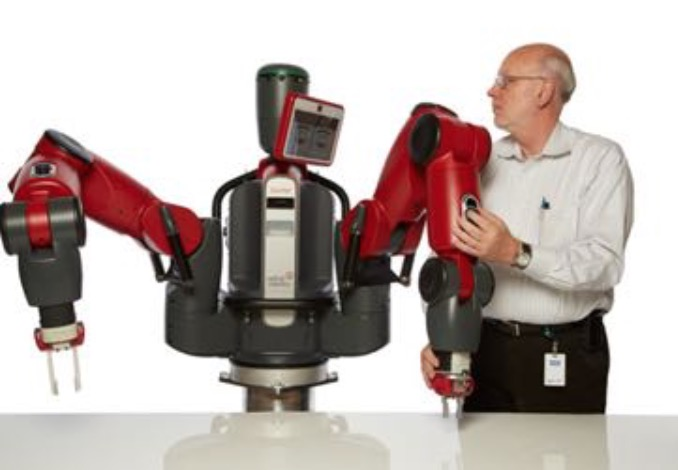
\includegraphics[scale=0.3]{./mypic/机器人示教非映射式.jpg} 
		\end{minipage}}
	\subfigure[机械臂映射式示教]{ 
		\begin{minipage}[b]{0.5\textwidth} 
		\centering
		% \label{fig:SubFigure1} %% label for second subfigure 
		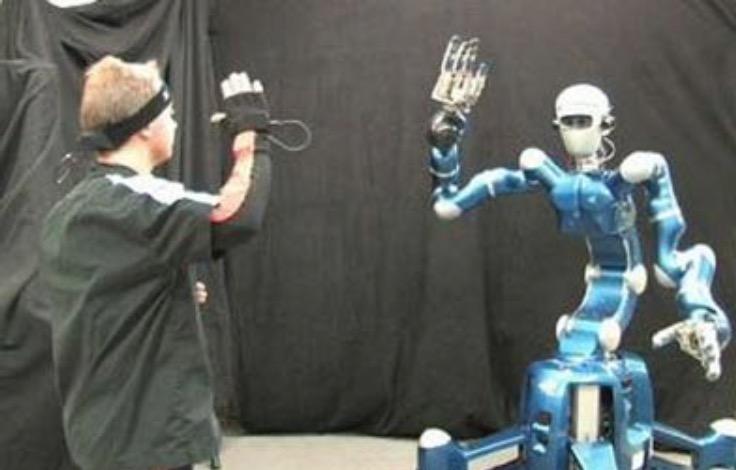
\includegraphics[scale=0.3]{./mypic/机器人示教映射式.jpg} 
		\end{minipage}}
	\caption{两种经典的演示编程示教方式}
\end{figure}

演示编程(Programming by Demonstration, 简称PbD)是目前工业研究一个非常前沿的话题,能够通过非常简单的操作方式降低工业机器人的操作复杂度。演示编程,也称为演示学习(Learning from Demonstation, 简称LfD),是由机器人系统从人的操作演示中提取理解有效信息,进而将该信息转化为机器人的程序和运动以及操作参数,从而使机器人完成相应的操作\cite{billard2008robot}。演示编程提供了一种新的向机器人传递信息的方式,是简化机器人编程的重要途径\cite{argall2009survey}。与传统机器人编程方法相比,它可以大大降低行业应用技术人员在机器人使用和编程方面所需的专业性知识要求,对于机器人的推广应用具有重要意义。但演示编程对机器人系统的智能性,特别是如何从人的操作演示中提取理解有效信息、并将该信息转化为可完成所要求作业任务的机器人程序,提出了巨大挑战。演示编程研究从上个世纪80年代中期开始,经过长期的研究,已经在运动轨迹学习领域取得了较为丰硕的成果,包括示教人演示动作的数据采集、映射和模型学习与泛化应用。上图为两种经典的演示编程示教方式。

对零件或者通用物体的位姿估计是众多演示编程示教任务中的一个基本核心任务。例如下图工业环节所示,需要将一些零件从传送带或者Tray盘上抓去抓取进行装配,或者放置到下一个工业环节中去,这其中就须要工业机器人知晓零件的位姿。通常传统方法是通过将零件整齐有规律地放置在一些有卡位结构的传送带或者Tray盘中,使得零件相对于工业机器人的位姿是绝对固定的。用这样的方法的确能直接解决问题,但同时也带来了例如机械臂标定,Tray盘传送带标定等一系列附加问题。并且这些标定问题通常是非常繁琐,非常浪费人力物力的。再加上目前由于工业场景是多变和复杂的,特别是柔性制造领域,工业零件也随着需求的变化而日新月异,一旦零件规格发生变化或是工艺发生了更新,所有的生产就会立马收到限制,极大降低了工业生产效率。但如果有一套高效便捷的零件位姿估计系统,就完全可以解决上述所有问题,大大降低生产空档时间,提升产出效率。因此对零件的位姿估计的研究具有非常高的工业应用价值和学术研究价值。因此本文将针对零件位姿估计展开研究。

\begin{figure}[htb]
	\subfigure[工业机器人抓取Tray盘上的零件]{ 
		\begin{minipage}[b]{0.5\textwidth} 
		\centering
		% \label{fig:SubFigure1} %% label for second subfigure 
		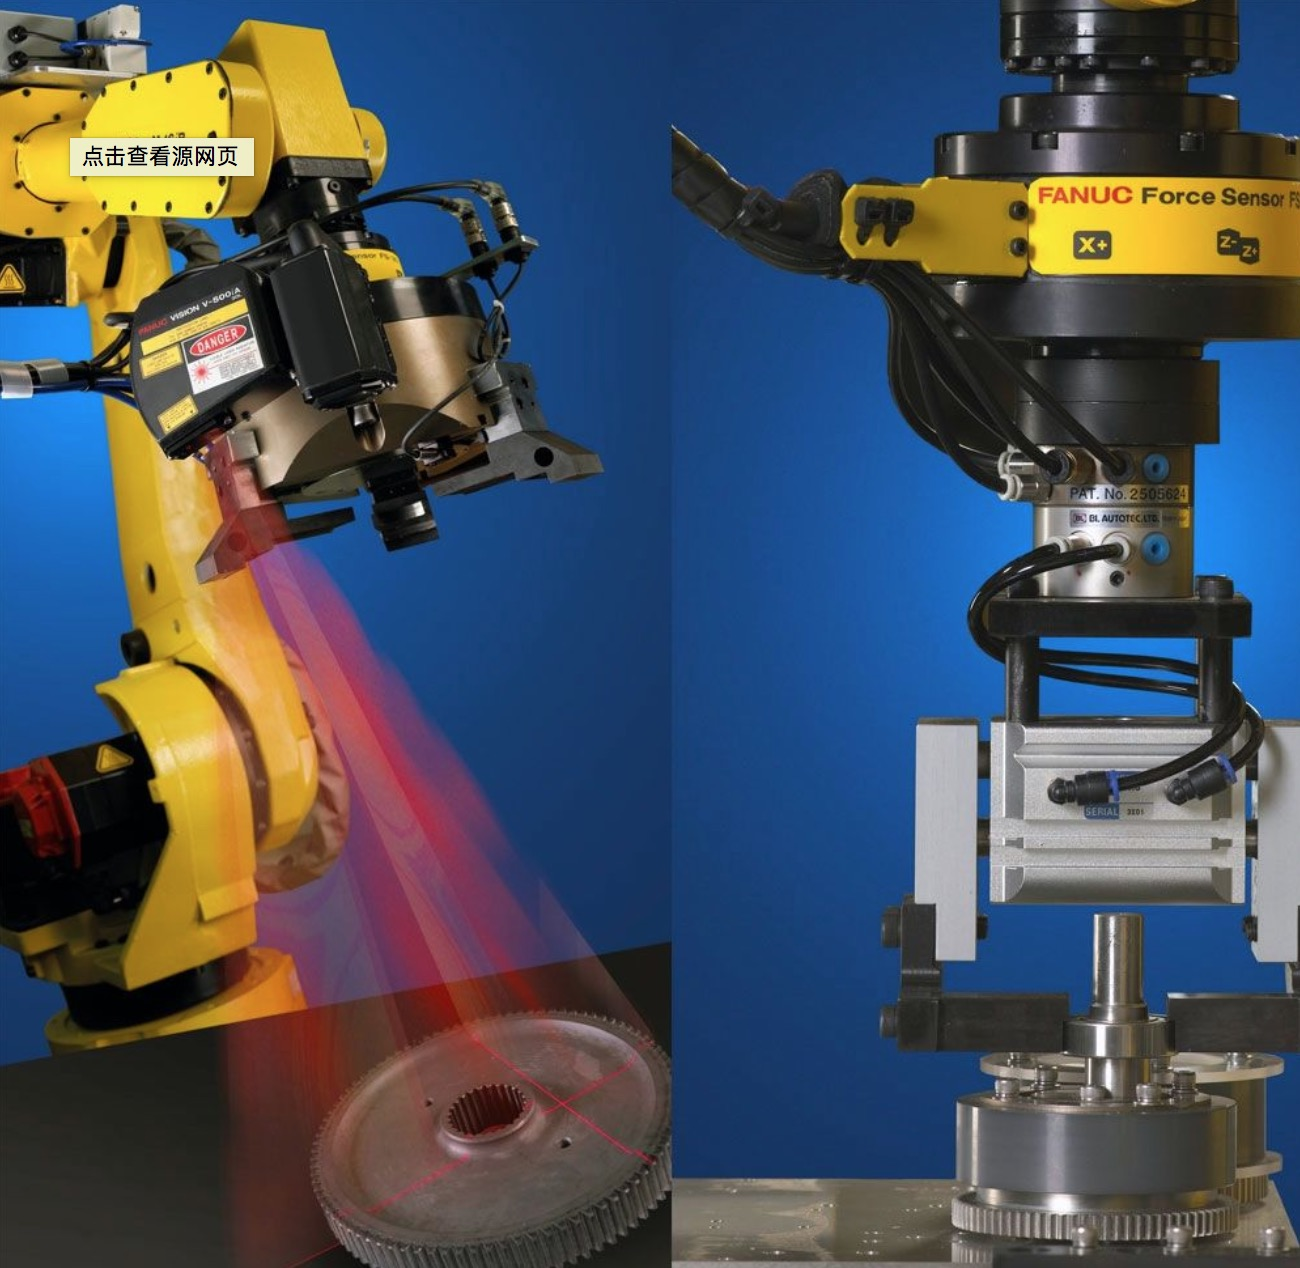
\includegraphics[scale=2.0]{./mypic/工业机器人2.jpg} 
		\end{minipage}}
	\subfigure[工业机器人抓取传送带盘上的零件]{ 
		\begin{minipage}[b]{0.5\textwidth} 
		\centering
		% \label{fig:SubFigure1} %% label for second subfigure 
		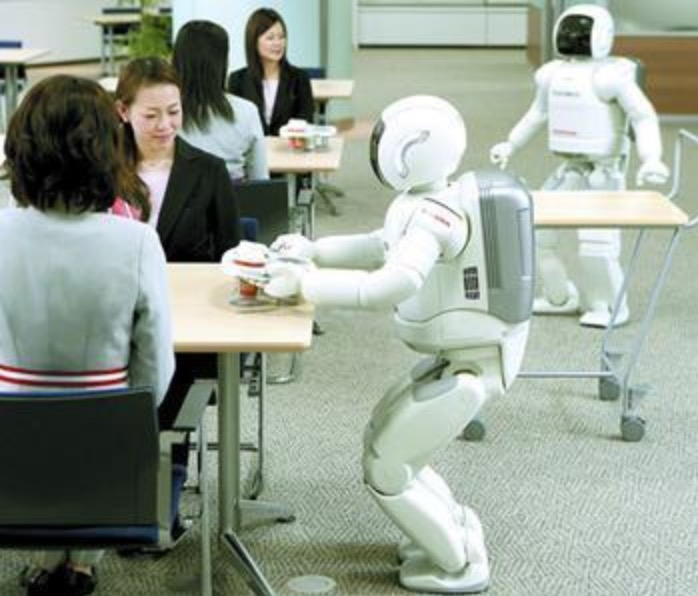
\includegraphics[scale=1.0]{./mypic/工业机器人1.jpg} 
		\end{minipage}}
	\caption{一些工业装配现场}
\end{figure}

在几乎所有工业环境中,计算机视觉是可以作为反馈的一种方便部署并且高效的方法。因此,计算机视觉已经成为了工业机器人研究领域中非常重要的一点。基于工业摄像头的计算机视觉是非常经典的研究内容,因为工业摄像头提供的高清RGB图像信息可以提供非常充足的环境信息,并且有很好的实时性。而近年来,伴随着例如Kinect,Leap Motion,RealSense等各种各样的面阵3D深度传感器的诞生,计算机视觉有了一个全新的维度。下图展示了一些常见的深度传感器。这些面阵3D深度传感器可以提供一个给定视角范围下工业场景的具有较高精度的深度尺寸信息,不再局限于只有RGB颜色信息的二维彩色图像上。并且这些3D深度传感器能在提供深度图像的同时给出与深度图像配准的RGB图像信息,也就是能够对空间中的物体同时进行颜色和深度的描述。这使得计算机视觉在感知上更接近于人眼,理论上可以观测到人眼所能观测到的所有信息。并且随着科技的发展,这些3D深度传感器的精度也在不断提高,传感范围也在不断扩大,其中Intel公司生产的RealSense传感器在近场工作环境下(20cm到120cm之间)精度可达1mm,完全可以应用于例如零件组装等特定工业场景中因此,针对这些3D深度传感器的计算机视觉研究掀起了一股热潮。

\begin{figure}[htb]
	\centering 
	% 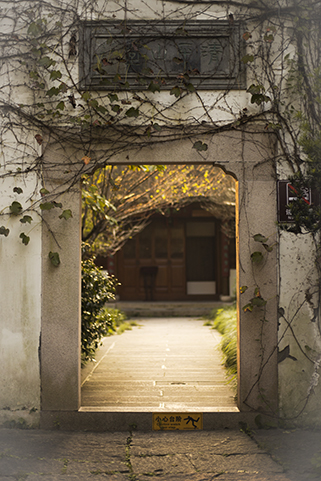
\includegraphics[width=\textwidth]{./Pictures/test.jpg} 
	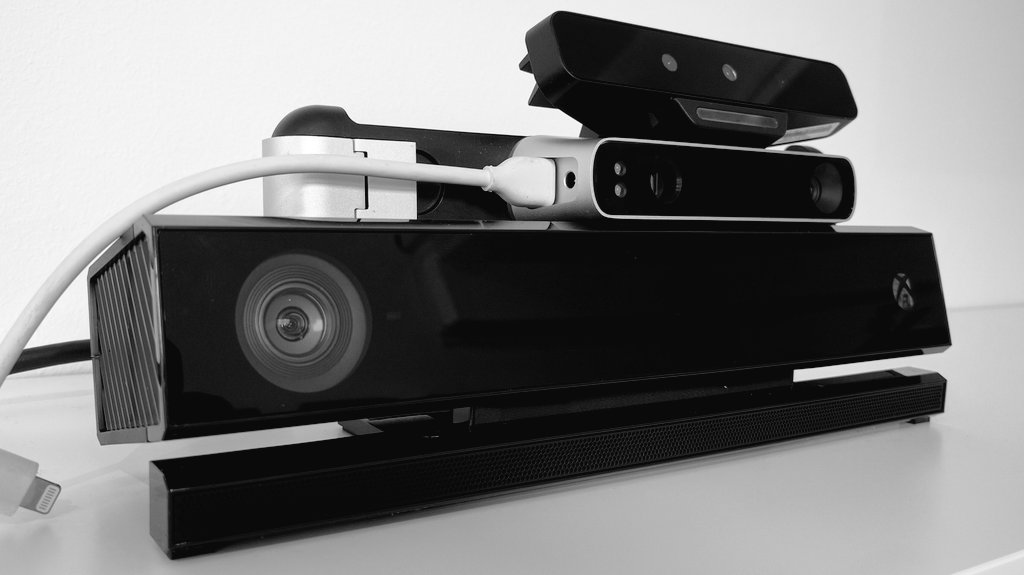
\includegraphics[width=0.8\textwidth]{./mypic/一些深度相机.jpg} 
	\caption{一些深度相机} 
\end{figure}


本文将在此背景下,面向工业装配演示编程中对物体位姿估计的需求,利用深度相机这一新型传感器展开研究和开发,以推动演示编程技术以及工业机器人的自动化发展。


\section{研究现状与趋势} 

物体位姿估计是一个非常大的领域。从目标角度来划分可以有人体姿势位姿估计、人脸特征点定位(五官位姿估计)、人脸朝向位姿估计、车牌位姿估计等各种其它实物的位姿估计。其中每一块内容都有非常多的研究人员投入,并且一直以来都有各种各样的方法和理论被提出,同时各个不同目标的位姿估计方法不断交融与碰撞产生更新颖更优秀的方法,持续促进着整个位姿估计领域整体的发展。但总体而言,物体位姿估计领域的各种优秀的方法可以被大致分为两种类型,一种是基于模版匹配的方法,另一种是基于模型回归的方法。两种方法各有优势也各有短处。

基于模版匹配的方法大致算法流程如下图所示。首先算法需要事先准备,或者事先计算好大量的模版,这些模版中每一个都代表被测物体的一个位姿状态。为了节省计算机资源和存储资源,这些模版在实际应用过程中将通过特征的形式进行存储,作为特征描述库。特征描述随算法不同而各不一样,常见的一些特征描述有SIFT\cite{lowe1999object},SURF\cite{bay2006surf},BRIEF\cite{calonder2010brief},ORB\cite{rublee2011orb}等经典特征描述。这些特征描述往往具有较好的尺度不变性以及对不同光照影响下的稳定性。存储好这些带有位姿信息等模版特征描述之后,便可以在实际位姿估计过程中通过比对输入的新图像的特征描述与特征描述库里的模版,得到一个最为接近的模版,从而最后得到对应的物体位姿。
\begin{figure}[htb]
	\centering 
	% 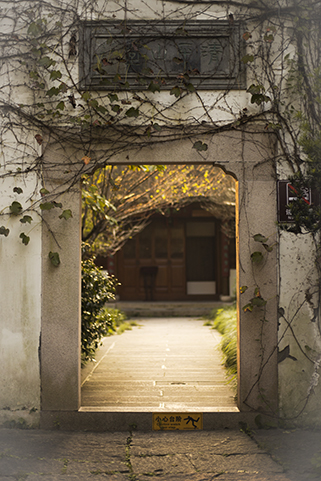
\includegraphics[width=\textwidth]{./Pictures/test.jpg} 
	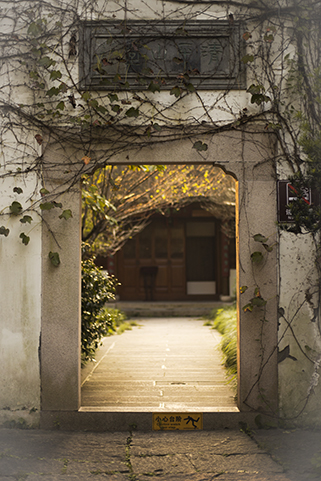
\includegraphics[scale=1.0]{./Pictures/test.jpg} 
	\caption{ljzst} 
\end{figure}

基于模型回归的位姿估计方法算法流程如下图所示。首先也是对目标物体进行特征提取,精准表达出物体的位姿特征。但是不同于基于模版匹配的算法框架,该方法在计算得到物体的特征描述之后不需要与实现准备好的模版库进行匹配,而是直接将位姿特征描述输入一个回归器里,通过回归器直接回归得到物体的位姿姿态。而其中这个位姿回归器则是通过事先大量的带真值标记的样本进行训练得到的。这其中的回归器可以是简单的线性回归,例如最小二乘回归等等,也可以是复杂的非线性回归例如SVM回归\cite{basak2007support}等。
\begin{figure}[htb]
	\centering 
	% 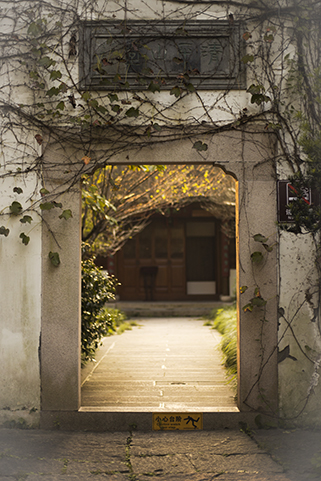
\includegraphics[width=\textwidth]{./Pictures/test.jpg} 
	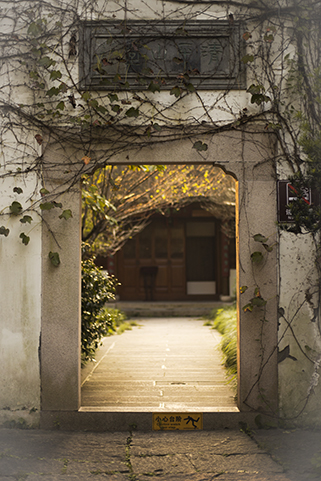
\includegraphics[scale=1.0]{./Pictures/test.jpg} 
	\caption{ljzst} 
\end{figure}

可以直观感受到,基于模版匹配的物体位姿估计方法通常需要较大的预存储空间,因为通常情况下一个物体的姿态会有非常大的变动空间,即使采用离散采样的方式来记录整个位姿空间下对应的各个位姿特征描述,也会有极大量的数据需要存储。一方面这样大量的存储会带来物理资源的需求,同时在进行位姿估计的过程中如果要匹配一对最接近的位姿特征描述,其计算量也是相当大的。相比之下基于模型回归的方法则有更为有竞争力。基于模型回归的方法虽然需要在事先通过学习大量的带标记的样本来得到物体的位姿回归器,但是位姿回归器在经过学习之后得到的模型通常只占有有非常小的数据存储空间。此外,当新的样本输入之后,位姿回归器根据其特征描述可以非常迅速地给出物体最终的位姿结果,不需要大量的计算资源。因此基于模型回归的位姿估计方法在实际应用过程中往往具有相对较强的竞争力。

在基于模型回归的位姿估计框架中,有很大一部分杰出的算法都用到了集成学习算法,并且考虑到位姿回归问题在回归空间上的高度复杂性,采用了非常新颖的级联回归算法进一步提高回归模型的回归能力。因此集成学习算法开始被大量关注并研究,同时级联回归算法框架也被不断应用到不同的领域当中。


\subsection{集成学习算法} % 随机森林与随机蕨 包括特征提取

集成学习方法通常指那些可以生成大量不同模型,并且可以将这些模型以一定的方式进行组合得到新的模型,从而用语解决分类或者回归问题\cite{mendes2012ensemble}。集成学习在很多情况下也被称为Committee、Classifier Fusion、Combination以及Aggregation等\cite{valentini2002ensembles}。从[\citenum{liu2000evolutionary}][\citenum{breiman2001random}][\citenum{rodriguez2006rotation}]等一些文章中可以看出,集成学习在近几年来取得了非常好的成绩,其优势具体表现在它相比单一的模型具有更加强大的鲁棒性以及准确性\cite{garcia2005cooperative}。其大致原理图如下所示:

\begin{figure}[htb]
	\centering 
	% 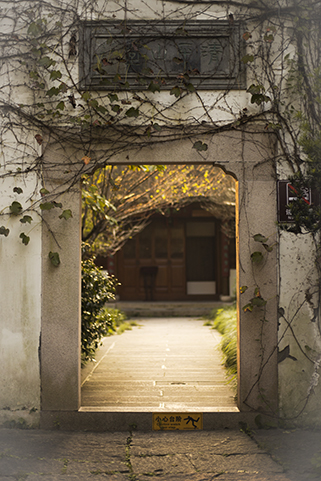
\includegraphics[width=\textwidth]{./Pictures/test.jpg} 
	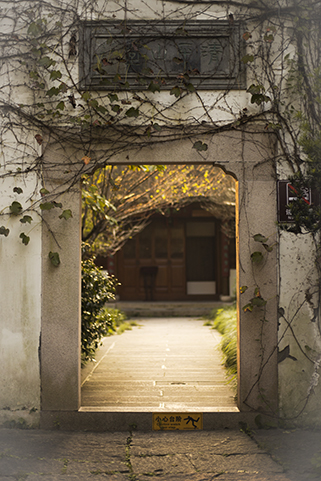
\includegraphics[scale=1.0]{./Pictures/test.jpg} 
	\caption{ljzst} 
\end{figure}


集成学习方法通过将不同模型进行组合得到新模型,按照这些子模型的种类关系可以将集成学习方法大致分为两种,分别是异态集成学习和同态集成学习。

异态集成学习是通过将种类不同的分类器进行集成,其中最为主要常见的两个主要方法为Wolpert等人提出的叠加法(Stack Generalization)\cite{wolpert1992stacked}以及Vilalta等人提出的元学习法(Meta Learning)\cite{vilalta2002perspective}。叠加法的思想是通过将基本的模型分布在多个层次上,再通过这个多层模型完成学习任务。William W等人在[\citenum{cohen2005stacked}]中则利用这种思想构造处了一种更加新颖的串行学习算法,并指出这种串行算法相比不串行在性能上有较大提升。元学习法的主要思想则是通过训练一个元模型来对所有的基本模型的输出进行进一步处理,最终得到问题输出结果。其主要包括两种方法:仲裁法(Arbiter)以及合并法(Combiner)。仲裁法是元模型从所有基本模型的输出结果中选择出合理的结果作为最后输出,例如投票方式。合并法则是通过用某种组合方法把所有基本模型的输出合并成最终输出,较为常见的Bagging\cite{breiman1996bagging}、Boosting\cite{schapire1990strength}等集成方法都是属于合并法。

同态集成学习方法则是指被集成的基本模型都应该属于同一种类的模型,仅仅只是这些基本模型之间的参数有所不同。同态集成学习模型主要有基于朴素贝叶斯的集成方法、基于决策树(Decision Tree,简称DT)的集成方法\cite{kearns1996boosting}、基于人工神经网络(Neuro-Network,简称NN)的集成方法\cite{zhou2002ensembling}\cite{zhou2002selectively}\cite{hansen1990neural}以及基于K—近邻的集成方法\cite{shen2007euk}等等。

异态集成学习方法由于需要提出众多不同模型才能构建更为强大的学习器,而通常情况下对于一个实际问题,要提出不同的模型来共同表述是一件非常困难的事情。相比之下,同态集成学习方法只需要提出一个简单的模型就可以完成复杂问题的学习。因此集成学习方法发展到现在,同态集成学习方法称为一种较为普遍并且表现优秀的一种学习方法,其中最为经典的一种同态集成学习方法就是随机森林\cite{breiman2001random}。随机森林算法是用随机的方式建立一个森林,森林里面有很多的决策树组成,随机森林的每一棵决策树之间是没有关联的。在得到森林之后,当有一个新的输入样本进入的时候,就让森林中的每一棵决策树分别进行一下判断,看看这个样本应该属于哪一类(对于分类算法),然后看看哪一类被选择最多,就预测这个样本为那一类。随机森林可以既可以处理属性为离散值的量,比如ID3算法,也可以处理属性为连续值的量,比如C4.5算法。另外,随机森林还可以用来进行无监督学习聚类和异常点检测。

与随机森林非常相似的另一个异态集成学习方法是随机蕨算法\cite{ozuysal2007fast}。随机蕨算法在2007年由Mustafa Ozuysal等人提出,并被广泛应用。其中最为出色的应用是在Zdenek Kalal等人提出的TLD跟踪算法中\cite{kalal2012tracking},该跟踪算法也称为深度学习大爆炸之前最为有名的跟踪算法之一。随机蕨算法表现出的优秀性质也被后来很多算法借鉴以及采用\cite{dollar2010cascaded}。

在众多优秀的集成学习算法中,本文希望能够挑选一种合适的学习算法,将其转变为适合物体位姿估计的集成学习方法。

\subsection{级联回归算法框架} % 人脸等在这里讲

在很多复杂回归问题中,级联回归算法是一种提高模型回归拟合能力的一种非常有效的方法。级联回归算法的初期想法由Jerome H Friedman等人在文章[\citenum{friedman2001greedy}]中提出。后来由Nigel Duffy等人经过研究在文章[\citenum{duffy2002boosting}]中进行了较为详细的叙述,将级联回归算法的核心思想以及能力进行了验证。随后经过大量的改进,SK Zhou等人将级联回归算法成功应用到了图像处理领域,这也奠定了之后一系列基于图像的级联回归处理算法基础\cite{zhou2005image}。

级联回归算法框架在各个应用场景下都得到了高度的认可,取得了不错的表现。在物体位姿估计领域,P. Doll{\'a}r等人在2010年提出了较为成熟稳定的一种物体位姿估计算法框架\cite{dollar2010cascaded}。在他们提出的文章中,采用了固定线性串流模型结构,通过将一系列回归器串联,每一级回归器充分利用上一层回归器的回归结果,不断补充回归器所能得到的输入信息,从而实现对回归目标更为精准的预测。如下图所示,首先算法需要一个目标所在的初始位姿,这个初始位姿不需要非常精准,然后算法通过对该初始位姿上的特征信息得到一个回归量用于矫正该初始位姿使其更加靠近真实位姿。
\begin{figure}[htb]
	\centering 
	% 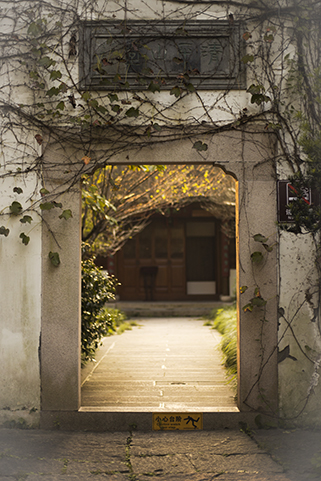
\includegraphics[width=\textwidth]{./Pictures/test.jpg} 
	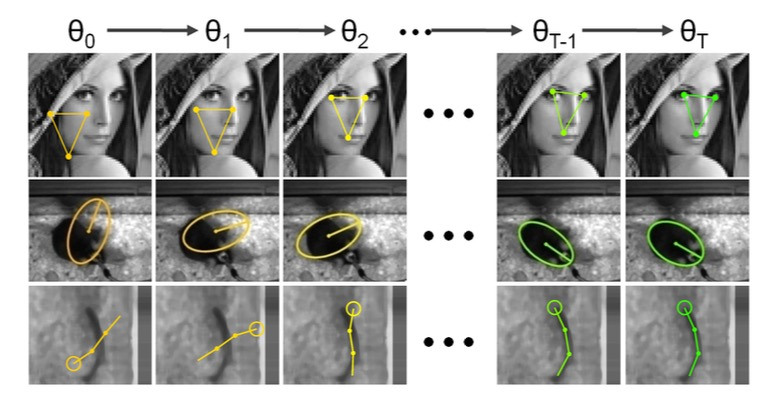
\includegraphics[width=\textwidth]{./mypic/级联回归.jpg} 
	\caption{图像上对物体位姿进行级联回归的一种基本框架} 
\end{figure}

级联回归算法在人脸特征点定位上取得的突破性进展是众多图像回归算法领域最为成功的一个。M. Dantone等人率先利用级联回归框架算法的高效性,并采用条件回归森林作为每一层的回归模型,得到了一种基于模型参数的实时人脸特征点定位算法,并取得了当时最精准的回归精度。同样借鉴于文章[\citenum{dollar2010cascaded}],X. Cao等人在2014年发表了一篇具有突破性意义的人脸特征点定位文章[\citenum{cao2014face}]。这篇文章中提出的人脸特征点回归算法采用非参数化的模型表达,通过直接估计人脸特征点在图像中的坐标位置来实现定位。这种通过直接减少特征点定位精度误差,而不是通过减少模型误差的方式,极大促进了回归精度以及回归速度。能有这样显著的效果提升,极大程度上依赖于级联回归框架的高拟合能力。随后P. Doll{\'a}r再一次总结X. Cao等人的工作经验,利用自己提出的级联回归框架,提出一种能够适应一定人脸被遮挡情况下的人脸特征点定位算法,再一次提高了人脸特征点定位的精准度\cite{burgos2013robust}。在期间也有相关的一些相关的神经网络回归算法被应用到这个领域,但是经过实验证明,神经网络的回归能力和级联回归算法框架下差别不大,但是在计算效率上则远不及级联回归算法\cite{sun2013deep},随后也被慢慢淘汰。最后在[\citenum{ren2014face}]文章中,R. Shaoqing等人提出了一种里程碑意义的人脸特征点定位算法。在该算法中,通过提出局部二值特征,并以级联回归学习框架对人脸特征进行学习,从而引导回归模型进行拟合,最后得到了具有极高精度,极高速度并存的人脸特征点定位算法。于此同时,类似文章[\citenum{cootes2001active}][\citenum{saragih2009face}][\citenum{yang2014face}][\citenum{asthana2014incremental}][\citenum{kazemi2014one}][\citenum{burgos2013robust}][\citenum{xiong2013supervised}]也通过类似的级联回归框架在人脸特征点定位领域取得了相当优秀的成果,具有很高学术借鉴意义。

人脸特征点级联回归回归算法的大致框架可以如下图所示:
\begin{figure}[htb]
	\centering 
	% 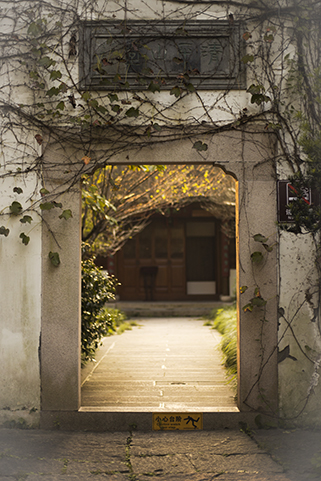
\includegraphics[width=\textwidth]{./Pictures/test.jpg} 
	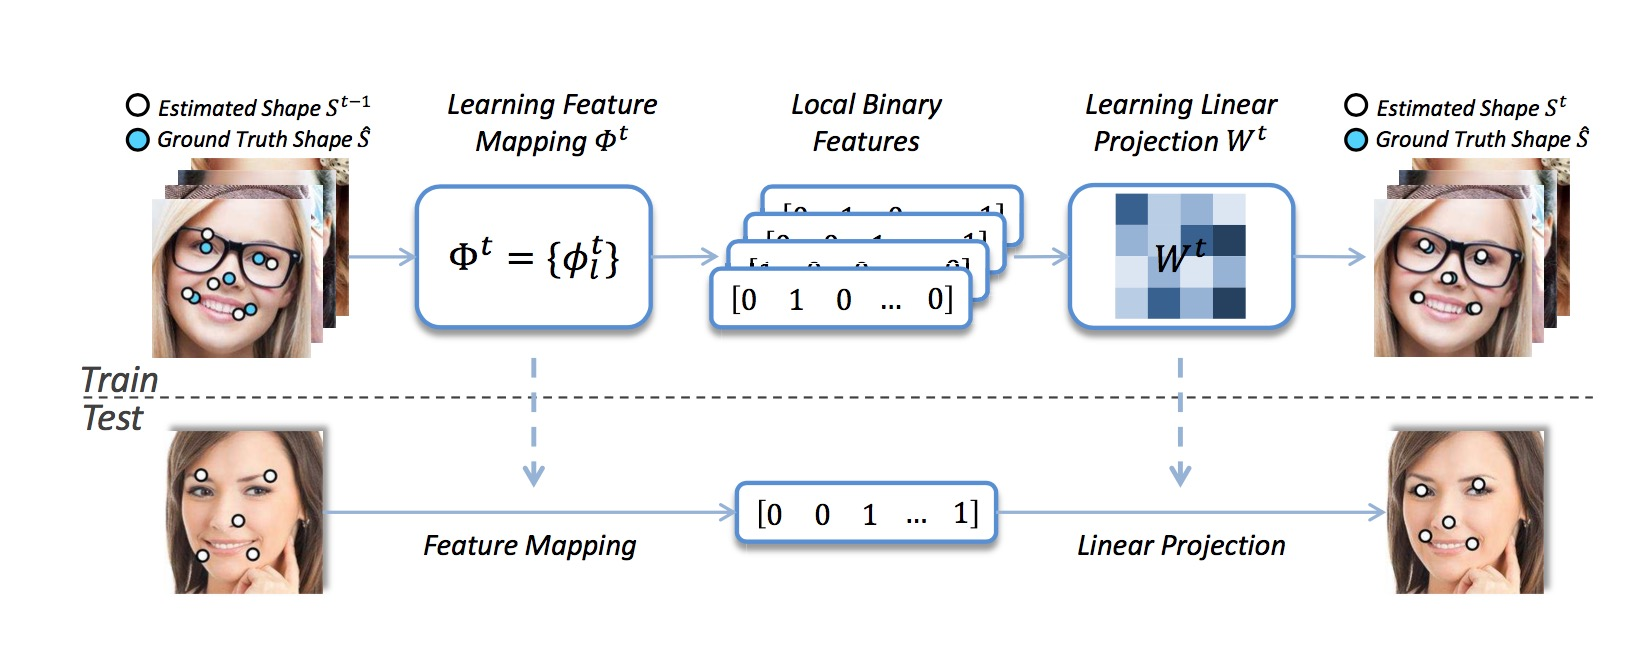
\includegraphics[width=\textwidth]{./mypic/人脸回归算法框架.jpg} 
	\caption{人脸特征点定位问题中的级联回归算法框架} 
\end{figure}
首先在训练模型阶段,学习计算出当前特征点处的特征描述,并以此作为下一级回归器的输入,而当前特征点位置与真值之间的偏移量作为下一级回归器的目标回归量。通过大量的真值样本进行训练得到下一级回归模型。此处特征点的位置可以由目标检测器初始化给出,或者是通过上一级的回归模型得到修正之后给出。重复上述过程就可以得到级联回归模型。而在实际测试应用中,通过计算当前特征点位置的特征描述作为当前级拟合回归模型的输入,得到当前目标回归矫正量。将该矫正量叠加到上级特征点位置后可以得到更新后的特征点位置。重复上述过程,完成所有级联回归模型的拟合修正就可以得到最后的人脸特征点位置。这样的模型非常简洁,但具有非常强的拟合能力,能够适应像人脸特征点定位这样具有非常高复杂度回归空间的回归问题,证明了级联回归模型具有相当优秀的实际应用价值。因此本文也希望充分利用这样的级联回归框架,对物体的六维位姿估计问题展开研究。

\subsection{物体的六维位姿估计}

物体的六维位姿估计一直以来是机器人领域一个基础问题。早期物体位姿估计的算法研究都是基于工业相机展开的。其中较为成功的几种算法有M. Jones提出的一种基于全局表面特征的位姿估计方法\cite{jones2003fast},以及一些基于局部表面特征的位姿估计方法\cite{schmid1996combining}\cite{rothganger20033d}。随后,D. Thachasongtham等人提出一种更为鲁棒的算法框架,通过事先仿真物体在三维空间中的各个位姿,并通过训练筛选出各个空间位姿下该物体具有的最为稳定的特征点以及相应的特征描述,最后在线测试时通过这些稳定的特征点进行三维位姿匹配\cite{thachasongtham20133d},这样的算法在当时具有一定的大角度变动适应性以及对一些遮挡情况有较好的表现。文章[\citenum{hara2014growing}]研发了一种增长回归随机森林用于对物体的位姿进行直接预测,但是该增长回归森林算法仅仅可用于分类问题,也就是对物体的直接位姿估计是不够精准的,需要后续其他迭代算法对其结果进行调优。

近些年来,随着深度相机的不断发展,各种新型的深度传感器给机器视觉带来了更丰富的信息来源,深度相机引发了一次物体位姿估计的研究热潮。文章[\citenum{germann2007automatic}]搭建了一个3D仿真环境,用于渲染3D模型在空间中的各个位姿,并利用这个仿真提取一些标准深度图像模版,最后通过在线匹配这些深度图像模版与实际深度相机采集到的深度图像进行位姿估计,初步实现了深度图像下的物体六维位姿估计。但由于这个版本的算法需要极大的计算量,文章作者利用GPU进行并行加速计算提高效率,但仍旧无法实现较快的结果输出。随后M. Germann等人改进了其算法,通过简化标准模版之间匹配的过程,同样利用GPU并行处理,提高了该算法框架的实时性,效果得到了显著提升\cite{park2010fast}。下图为该类算法一个简易框架示意图,其中最后调优过程一般采用ICP(Iterative Closest Point)算法。
\begin{figure}[htb]
	\centering 
	% 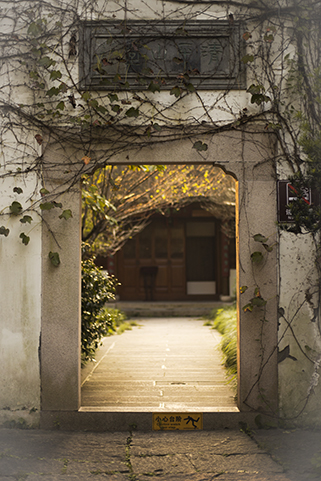
\includegraphics[width=\textwidth]{./Pictures/test.jpg} 
	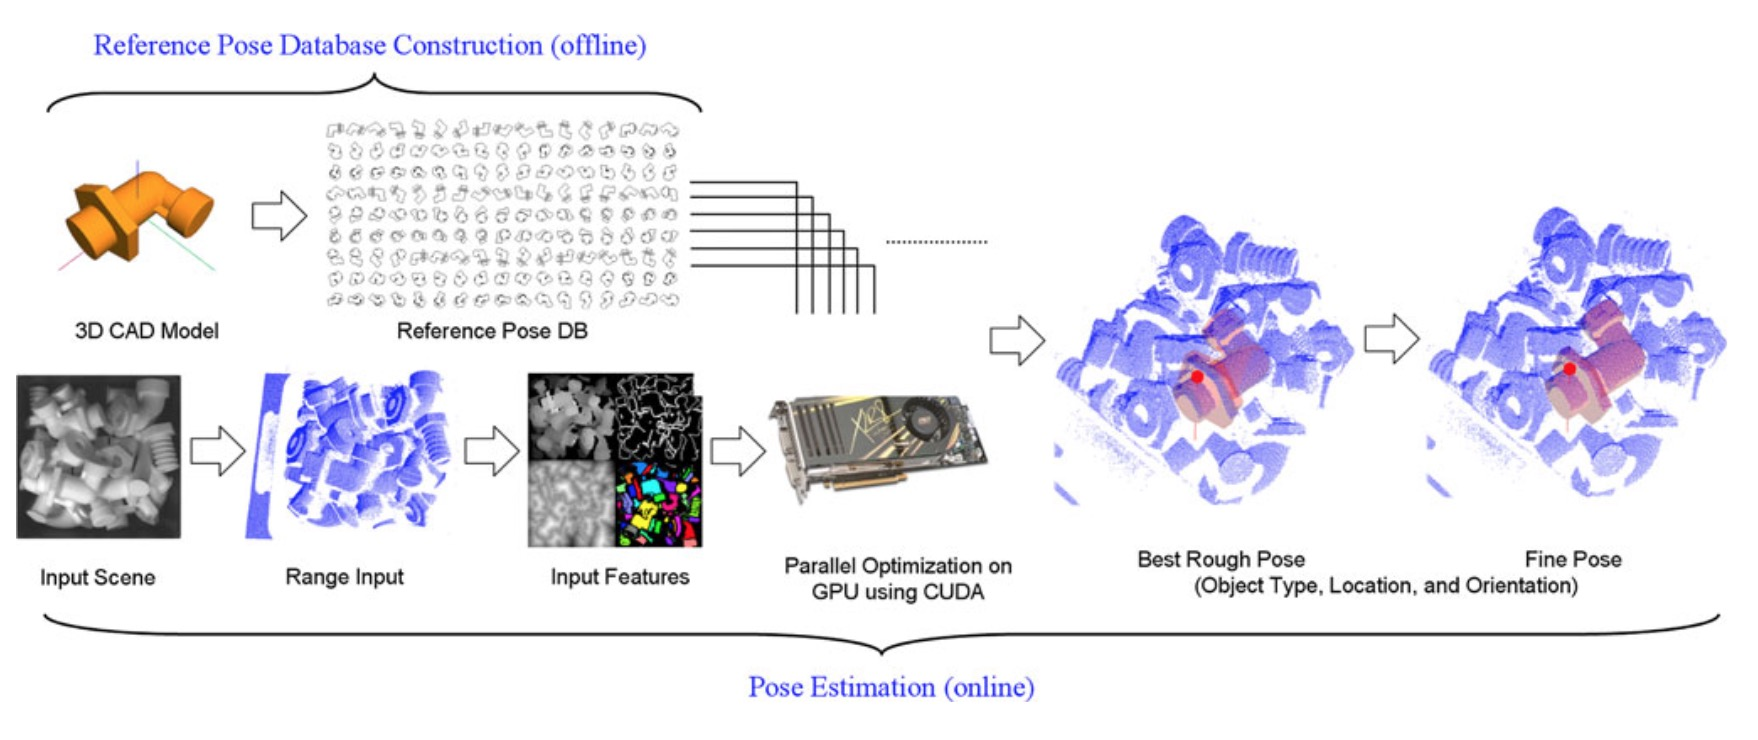
\includegraphics[width=\textwidth]{./mypic/早期位姿估计算法框架.jpg} 
	\caption{早期位姿估计算法框架} 
\end{figure}

为了提高物体位姿估计的实时性,B. Drost等人提出一种基于点云法向量的全局模型特征PPF(Point Pair Features)。这种特征包含了所有模型点云对之间的特性并且与整个模型之间存在一种配对关系,同时具有非常好的计算效率\cite{drost2010model}。利用这种特征描述进行投票机制的位姿估计,使其算法具有非常好的速度以及精度表现。另外S. Hinterstoisser等人则直接利用深度图像计算其对应的梯度响应图作为其特征匹配的基础,得到了非常好的位姿估计效果,同时其计算实时性也非常高\cite{hinterstoisser2012gradient}。他们提出了一种叫做LINE(LINEearizing the memory)特征,包含仅用于深度图像的LINE-2D特征、用于深度图像表面法向量的LINE-3D特征以及用于多模型的LINE-MOD特征。这些特征描述具有非常好的表达能力,是深度图像特征中非常实用的方法。之后他们利用这些特征又提出了一种多模版匹配算法,用于复杂环境下的物体位姿估计,并取得了相当好的效果\cite{hinterstoisser2011multimodal}。

在文章[\citenum{tang2014latent}]提出潜回归随机森林以及文章[\citenum{gall2011hough}]提出霍夫随机森林这两个相当优秀的回归森林算法之后,A. Tejani等人结合这两种算法,提出一种新颖的潜类别霍夫随机森林算法,同时结合LINE-MOD特征用于物体的检测以及六维位姿估计\cite{tejani2014latent}。该算法在当时表现相当出色,取得了State-of-the-art效果。于此同时,E. Brachmann等人采用能量谱图结合随机森林投票的方式也取得了不错的结果,具有较好的借鉴意义\cite{brachmann2014learning}。

随着深度学习的出现和流行,一些基于深度学习的物体位姿框架也逐渐被提出。P. Wohlhart等人提出的一种深度学习特征提取框架能够得到相比LINE-MOD特征更好的特征表述\cite{wohlhart2015learning}。但受限于深度学习框架的庞大性,很难实现高效便捷的算法部署,因此类似的利用深度学习框架进行位姿估计的算法研究成果大都不是特别理想。

得益于人脸特征点定位取得的优秀成果,X. Sun等人将人脸特征点定位算法进行移植改造应用于人手掌的位姿估计中,取得了相当优秀的成果\cite{sun2015cascaded}。该算法通过给手掌指定一些关键点,并设计了一种能适用于深度图像的特征描述方式进行级联回归,能够在不利用GPU并行加速计算的情况下对手掌进行实时位姿估计,同时具备相当准确的位姿回归精度。下图是该算法的一个简单流程示意图:
\begin{figure}[htb]
	\centering 
	% 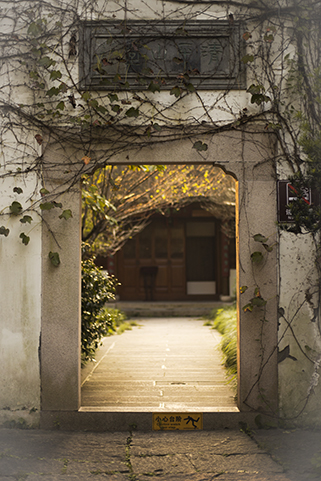
\includegraphics[width=\textwidth]{./Pictures/test.jpg} 
	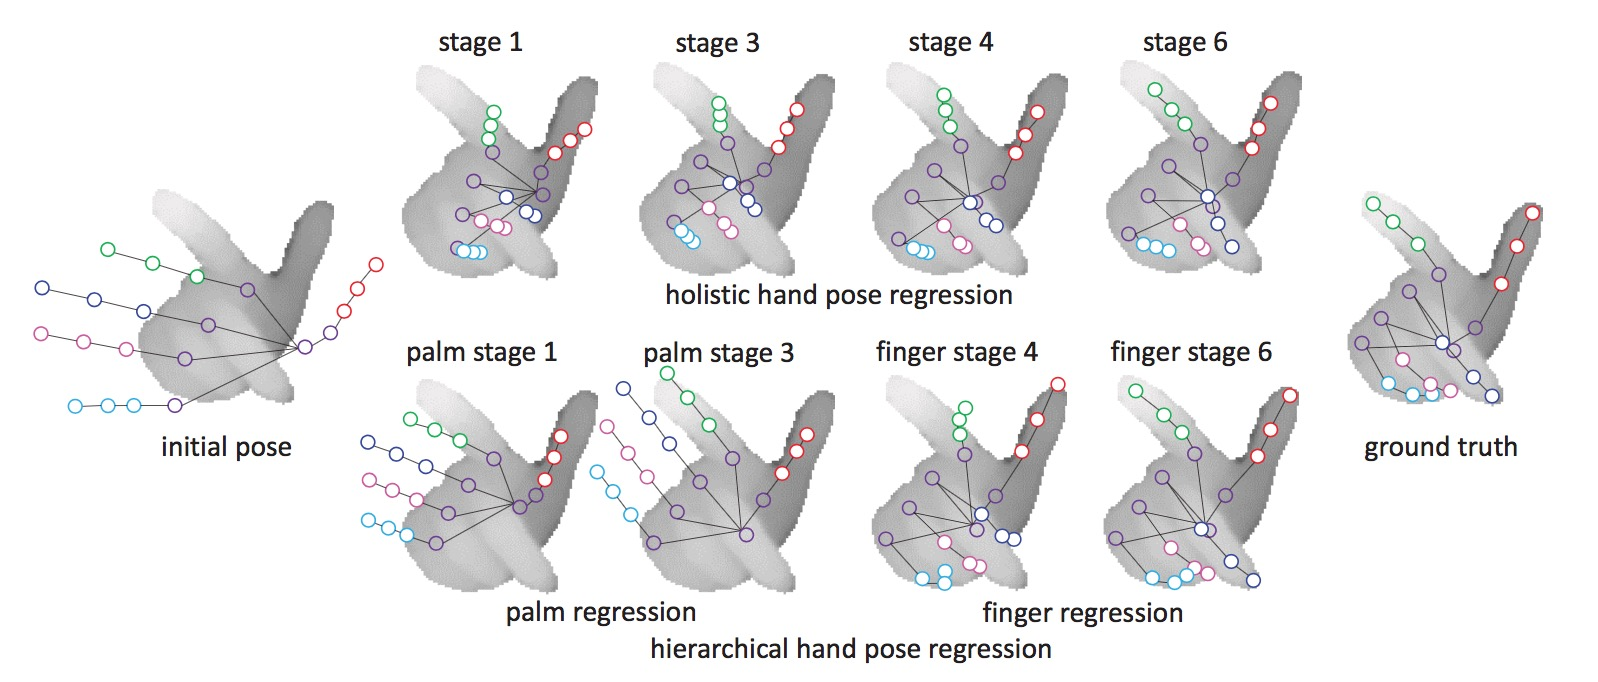
\includegraphics[width=\textwidth]{./mypic/手掌位姿估计流程示意图.jpg} 
	\caption{手掌位姿估计流程示意图} 
\end{figure}
首先在深度图像中给定一个任意的手掌初始位姿,然后通过对关键点的深度图像特征提取,结合随机森林算法进行级联回归最后得到准确的手掌位姿。类似的,E. Brachmann也采用了级联回归框架进行了对通用物体的位姿估计研究,采用RGBD相机作为借口实现了较为理想的位姿估计结果,但在计算效率上略有降低\cite{brachmann2016uncertainty}。这些工作指引物体位姿估计研究的重点放在了级联回归框架上,随后R. Kouskouridas等人进一步改进潜类别霍夫随机森林,实现了物体六维位姿估计高精度情况下的又一次性能提升\cite{kouskouridas2016latent}。

总体而言,物体位姿估计研究在朝着高效率高精度的方向发展。但首先于目前深度相机的精度还并没有非常高,所以目前的研究主要是通过改进算法框架,实现一个更易部署,更为高速的物体位姿估计算法。因此文本也希望能够进一步提高物体位姿估计算法的效率,同时保证其有较好的精度。

\section{本文研究内容}

工业装配演示编程的背景下,物体的六维位姿估计研究具有如下几个特点:
\begin{itemize}
\item 工业现场需要进行物体位姿估计的场合中,这些物体往往是具有严格尺寸信息的规则刚体,一般都有精确的3D模型。
\item 工业现场很多零件日新月异,每当有一个新的零件需要投入生产时都需要对流水线过程进行更新,或者物体位姿估计算法更新。
\item 工业现场追求效率,所有的应用算法都需要有较高的实时性从而提高生产效率。
\end{itemize}
针对上述这几个现实问题,本文思路为通过继续深入研究随机森林等集成学习算法,进一步提高这类算法的适用性以及鲁棒性,从而使其应用于物体位姿估计领域时能有更好的表现。另一方面为了使物体位姿估计算法具有更好的通用性以及更好的易部署性,本文将考虑利用现有工业条件搭建一个物理仿真环境,方便物体位姿估计算法的快速实现。最后结合级联回归框架得到一个较为完善的工业场景下的物体六维位姿估计方案。

本文最终得到的研究内容可以分为下面这三个大块:
\begin{itemize}
\item 首先以人脸特征点定位这个较为成熟的研究平台来验证随机蕨回归算法的可靠性,以及随机蕨回归算法在面对高维回归空间问题的回归能力和效率。并通过修改经典随机蕨回归框架,通过给算法输入增加一个掩码接口,实现随机蕨回归算法能够有更强的适应性,在针对特征不完备情况下的回归也能合理进行。最后通过实验验证该算法的可行性。
\item 充分利用工业现场可以提供的零件的3D模型信息,借助OpenGL软件平台搭建一个深度相机仿真平台。通过模拟零件在相机视角下的各个位姿,并添加对应的背景以及前景信息,在短时间内生成大量的仿真数据用于后续对物体位姿估计模型的训练。同时,本文将通过修补深度相机产生的空洞以及为仿真深度图像添加随机噪声使其与真实深度图像更为接近,提高仿真程度。
\item 借鉴人脸特征点定位以及文章[\citenum{sun2015cascaded}]中的思路,针对工业现场零件的位姿估计问题设计全新的物体六维位姿级联回归算法框架。并通过设计新的深度图像特征实现物体六维位姿估计算法的高效性。最后利用改进后的随机蕨回归算法,通过对物体的遮挡情况进行估计,实现当物体存在部分被遮挡情况下也能得到较为理想的物体位姿估计结果。
\end{itemize}


\section{本文结构安排}

本文结构安排如下:

第一章主要介绍了在工业环境下本文针对物体位姿估计研究的背景以及意义,并给出了当前集成学习、级联回归算法以及物体六维位姿估计等领域的研究现状。随后给出了本文的主要研究内容以及结构安排。

第二章中先给出了随机蕨算法的经典定义,并通过改造随机蕨算法中的推理公式改造为可以用于回归问题的随机蕨回归算法。然后结合实际应用问题,进一步改造随机蕨算法将其结合特征掩码,介绍如何将随机蕨算法应用到有大噪声干扰的情况中去。最后通过实验验证这些算法改进之后的合理性以及可行性。

第三章主要介绍了在搭建仿真深度相机过程中的数学模型,以及仿真环境搭建的主要流程。其中包括仿真环境中的坐标系设定、旋转关系、OpenGL中的一些基本原理等。并通过进一步为仿真深度图添加人工噪声以及前景背景信息增强其仿真真实度。最后在实验中给出仿真环境的一系列结果。

第四章首先提出了一种可以用于深度图像上的特征提取办法,讨论其尺度不变性,并利用一种监督学习下的特征降维办法对特征进行信噪比提高。然后针对物体的位姿估计提出一种级联回归框架,使其能够实现对通用物体的六维位姿估计。接着进一步讨论物体在存在遮挡情况下如何利用扩展功能后的随机蕨进行针对性处理,以实现复杂环境下的物体位姿估计。最后在本章实验环节中给出了该物体位姿估计算法的可行性以及准确性分析。

第五章给出了本文研究过程中的一些总结,以及对之后的研究工作作出展望。















\chapter{随机蕨算法的改造与应用}

\section{概述}

随机蕨算法是随机森林算法的一种变种,也是基于传统贝叶斯理论提出的一种集成学习方法,
最早由Mustafa Ozuysal等人提出\cite{ozuysal2007fast}。
随机蕨和随机森林的区别主要有如下这四个方面:
\begin{itemize}
\item
随机森林算法直接学习后验概率,
而随机蕨算法则是通过学习类别条件概率密度分布
\item
在随机森林算法中,对于每个输入样本,比较的特征次序会有所不同,
但是在随机蕨算法中,对于每个输入的样本比较的特征的次序都是相同的。
\item
在训练过程中,随机森林算法的训练时间是随着随机树的深度指数增长,
而在随机蕨算法中,训练时间仅仅随着数的深度呈线性增长。
\item
在随机森林算法中,算法的最后结果是通过对每个决策树的加权平均来得到的,但是在随机蕨算法中,最后结果则是以贝叶斯规则综合得到。
\end{itemize}
% \begin{itemize}
% \item
% 随机森林算法直接学习后验概率$P(C_k|F)$,
% 而随机蕨算法则是通过学习类别条件概率密度分布$P(F|C_k)$
% \item
% 在随机森林算法中,对于每个输入样本,比较的特征次序会有所不同,
% 但是在随机蕨算法中,对于每个输入的样本比较的特征的次序都是相同的。
% \item
% 在训练过程中,随机森林算法的训练时间是随着随机树的深度指数增长,
% 而在随机蕨算法中,训练时间仅仅随着数的深度呈线性增长。
% \item
% 在随机森林算法中,算法的最后结果是通过对每个决策树的加权平均来得到的,但是在随机蕨算法中,最后结果则是以贝叶斯规则综合得到。
% \end{itemize}
% 其中,$P$表述算法最后的概率输出结果,$C_k$表示算法分类器的目标类别,$F=\{f_1,f_2,...,f_N\}$表示输入算法的特征,下文同。
随机蕨算法经过实验验证,在相同层数的情况下,具有比随机森林更为优秀的分类能力以及抗过拟合能力,同时在计算效率上与随机森林不分上下,仅仅在模型存储上有较高的需求。因此随机蕨凭借出色的表现,得到了越来越多的关注。

但随机蕨算法目前的讨论都是在分类问题的基础上进行的,算法最后的结果也是在给定类别数目的情况下才能实现。但是在很多实际问题中,往往遇到的是回归问题,需要求解的目标空间往往是连续的,这个时候上述方法将不再适用。本文针对这样的情况,结合随机蕨的特性,借鉴随机森林算法改造应用到拟合回归问题中的方法,将随机蕨算法加以改造,使其也能适用于拟合回归问题。在此基础上,本文将进一步扩充随机蕨算法,通过增加一层掩码机制使其在输入特征有较大噪声的情况下也能有较强的鲁棒性,使算法能够在更多的应用场景中有更稳定的表现。

本章结构安排如下:节2.2介绍随机蕨算法通过修改输出函数表达式可以实现其在拟合回归问题中的应用。节2.3将介绍如何将掩码添加进随机蕨算法框架中,从而实现随机蕨算法在对抗大噪声情况下仍然具有较强的鲁棒性。最后在节2.4,本文通过将随机蕨算法应用到人脸对齐问题中,通过实验验证了改进后的随机蕨算法在回归问题中的可行性以及相比于普通拟合算法的鲁棒性,说明了该改进算法具有较强的实用性。



\section{随机蕨算法基本原理}
本节简要阐述一下随机蕨算法的具体原理。对于一个分类问题,需要计算各个类别间的概率分布:
\begin{equation}
	\arg\max_{k} P(C_k|f_1,f_2,...,f_N)
\end{equation}
其中,$P$表述算法最后的概率输出结果,$C_k$表示算法分类器的目标类别,$F=\{f_1,f_2,...,f_N\}$表示输入算法的特征。在贝叶斯规则下,上式等价于:
\begin{equation}
	\arg\max_{k} P(f_1,f_2,...,f_N|C_k)P(C_k)
\end{equation}
该式子表明一个后验概率与先验概率密度与相似函数的乘积成正比。然而对于一个高纬度的特征描述,或者说一个复杂的决策树输入样本,是很难计算出或者学习出相关联的相似度分布。或者说计算高维度的相似度分布是一件非常耗时耗资源的工作,在很多计算资源有限、计算实时要求高的应用场景中,计算高维特征相似度变得非常笨重,$P(f_1,f_2,...,f_N|C_k)$会非常难以求解。但如果假设在给定了目标类别的情况下,特征的各个维度之间是有一定的相互独立性的。这个时候,朴素贝叶斯理论可以对上述公式有如下简化:
\begin{equation}
	P(f_1,f_2,...,f_N|C_k)=\prod_{i=1}^N P(f_i|C_k)
\end{equation}
从而目标类别表达式为:
\begin{equation}
	Class(F)\equiv \arg\max_k P(C_k)\prod_{n=1}^N P(f_n|C_k)
\end{equation}
但这个独立性的假设在大多数的情况下是很难成立的,大多数情况下,上式得到的概率结果会小于真实的后验概率。为此,需要进一步假设。假设高维特征可以分解为几个小特征组合,并且这些小的特征组合之间是几乎完全相互独立的。这个假设在很多情况下都可以满足实用性。例如原始特征$F$分解为L组,每一组的特征大小为S,则有:
\begin{equation}
\begin{aligned}
	F=\{F_1,F_2,...,F_L\} \\
% \end{equation}
% \begin{equation}
	F_l=\{f_{l_1},f_{l_2},...,f_{l_S}\}
\end{aligned}
\end{equation}
当L组特征间相互独立假设下:
\begin{equation}
	P(f_1,f_2,...,f_N|C_k)=\prod_{l=1}^L P(F_l|C_k)
\end{equation}
于是可以得到最后的类别概率分布:
\begin{equation}
	Class(F_l)\equiv \arg\max_k P(C_k)\prod_{l=1}^L P(F_l|C_k)
\end{equation}
上式就是随机蕨算法的根本,采用半朴素贝叶斯的方式,平衡了算法计算的复杂性以及算法的准确性。其中每一个特征组构成的决策树被称为一个蕨,实际应用过程中,通过调整蕨的大小(也就是$S$的大小),就可以实现对算法复杂性以及准确性的控制。图2-1为该经典随机蕨算法的示意图。
\begin{figure}[htb]
	\centering 
	% 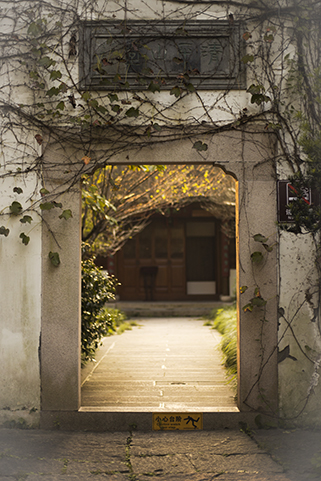
\includegraphics[width=\textwidth]{./Pictures/test.jpg} 
	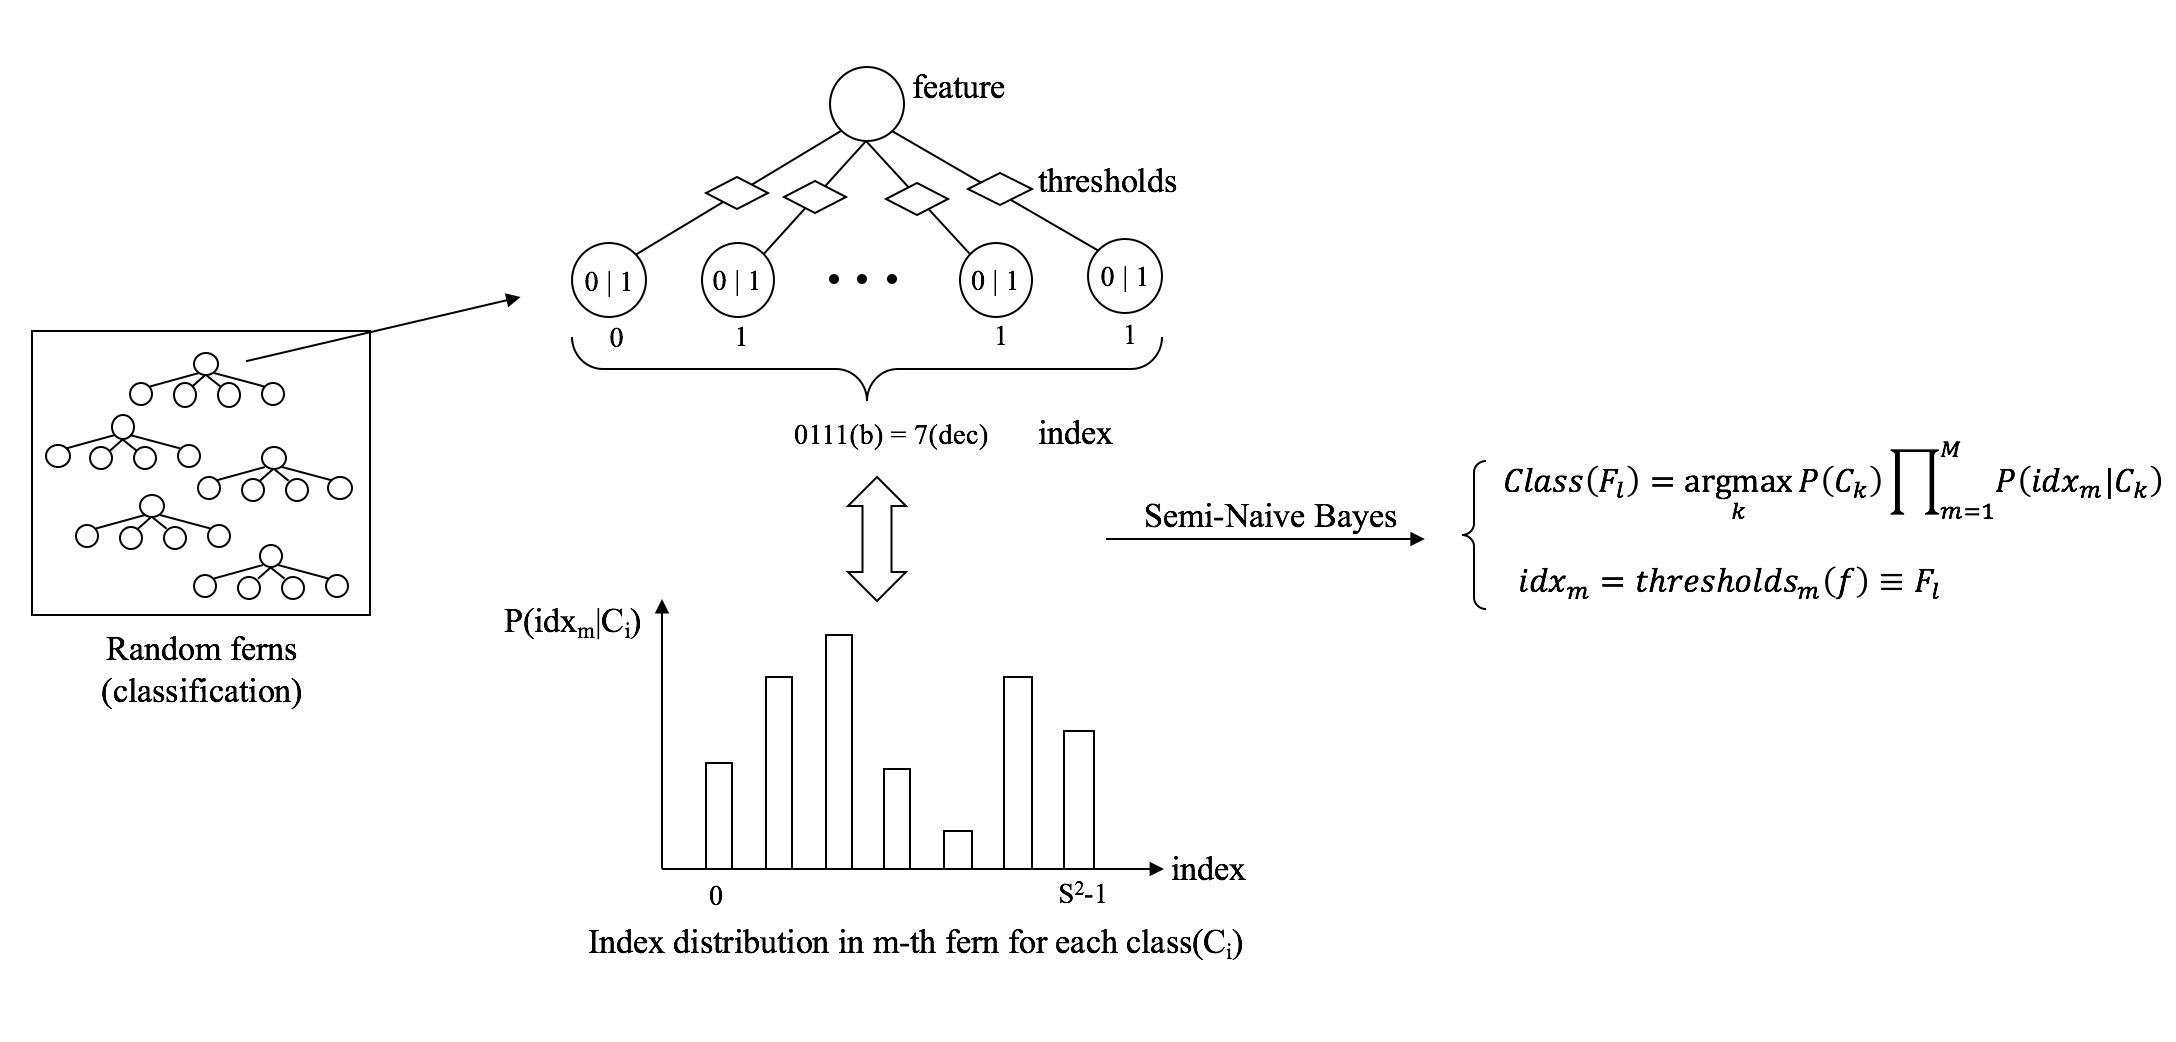
\includegraphics[width=\textwidth]{./mypic/经典随机蕨算法的示意图.jpg} 
	\caption{面向分类问题的经典随机蕨算法示意图} 
\end{figure}



\section{拟合回归问题下的随机蕨算法}
在分类问题下的随机蕨算法中,每个决策树的叶子节点记录的是所有落到该叶子节点的样本的类别概率分布均值。该模型在遇到新的输入样本后,将根据样本最后落入的叶子节点,统计所有叶子节点的概率分布均值来计算该样本的最后分类结果。这个模型显然不适用于回归问题。随机蕨算法被用于解决回归问题的思想最早在文章[\citenum{dollar2010cascaded}]中提出,后来也被应用到人脸对齐问题中\cite{cao2014face},但是都没有对其进行详细的说明阐述,很多算法实现细节被隐藏了。因此,本文将根据自己的理解和对算法的改善在此重新整理。

假定所有的输入样本都具有相同的特征维度$N$,$F=\{f_1,f_2,...,f_N\}$,以及相同$P$维度的目标回归空间$Y=\{y_1,y_2,...,y_P\}$。

首先任意地随机选取$S$个输入特征维度$(S<N)$,并随机生成$S$个阈值。将训练数据的这$S$个维度与这$S$个随机阈值进行简单大小比较,理想情况下可以得到$2^S$种不同的情况,同时对应地生成$2^S$个索引码。对这$2^S$个类别下的训练数据,我们计算其类内的均值,并记录为$L:\{L_1,L_2,...,L_{2^S}\}$,这样我们就得到了一个最简单的蕨。对于这个蕨,每次输入一个新的样本,仅仅需要将这个新的样本中那对应的$S$个维度上的数值与这$S$个阈值进行比较,就可以得到一个分类索引,然后只要根据这个索引在$L$中找到对应的均值记录(假定索引值为$i$),取出该均值便可以得到新样本的回归拟合值$L_i$。

这个基础蕨具有非常弱的拟合能力,甚至在随机阈值非常极端的情况下有可能完全不具备拟合能力。因此,我们需要重复这个随机过程(包括选取随机维度和生产随机阈值)多次,并记录下每一次随机过程的结果,并用损失函数来衡量这个随机过程得到的基础蕨的质量。损失函数可以有很多,例如:
\begin{equation}
	Loss=\sum_i{\|L_i-\overline{L_i}\|}
\end{equation}
如果某一次得到的损失函数值在所有随机过程中为最小,则抛弃所有其它的随机过程,用这次随机过程中选取的随机维度和随机阈值作为这个基础蕨的最终模型。记录维度信息$dim$、阈值信息$thresh$以及该阈值下的样本类别均值$L$。

这样的重复随机过程在经历一定量的次数之后将会大大加强该基础随机蕨的拟合能力,但是受限于随机过程的可重复次数,以及基础蕨的分类能力仅仅能实现$2^S$个,也限制了该基础蕨的拟合能力上限。因此,为了继续提高随机蕨算法的拟合能力,需要增加这种基础蕨的数量。区别于随机森林算法中各个树之间是相互独立的,随机蕨在生成众多的基础蕨过程中是有相互继承关系的。第一个基础蕨可以按上文所述进行生成,当生成第二个以及之后的基础蕨时,需要对每个样本的回归目标值进行修正,修正量就是上层基础随机蕨的预测结果。也就是说,第k层的回归目标值需要更新为:
\begin{equation}
	Y_{new}=Y_{original}-\sum_{i=0}^{k-1} Y_{pred_i}
\end{equation}
更新目标回归值之后,继续训练一定层数的随机蕨之后就可以得到最后具有非常高拟合能力的随机蕨模型。图2-2为该改进后的随机蕨回归算法的流程示意图。
\begin{figure}[htb]
	\centering 
	% 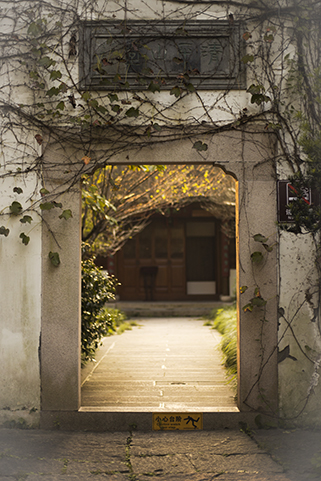
\includegraphics[width=\textwidth]{./Pictures/test.jpg} 
	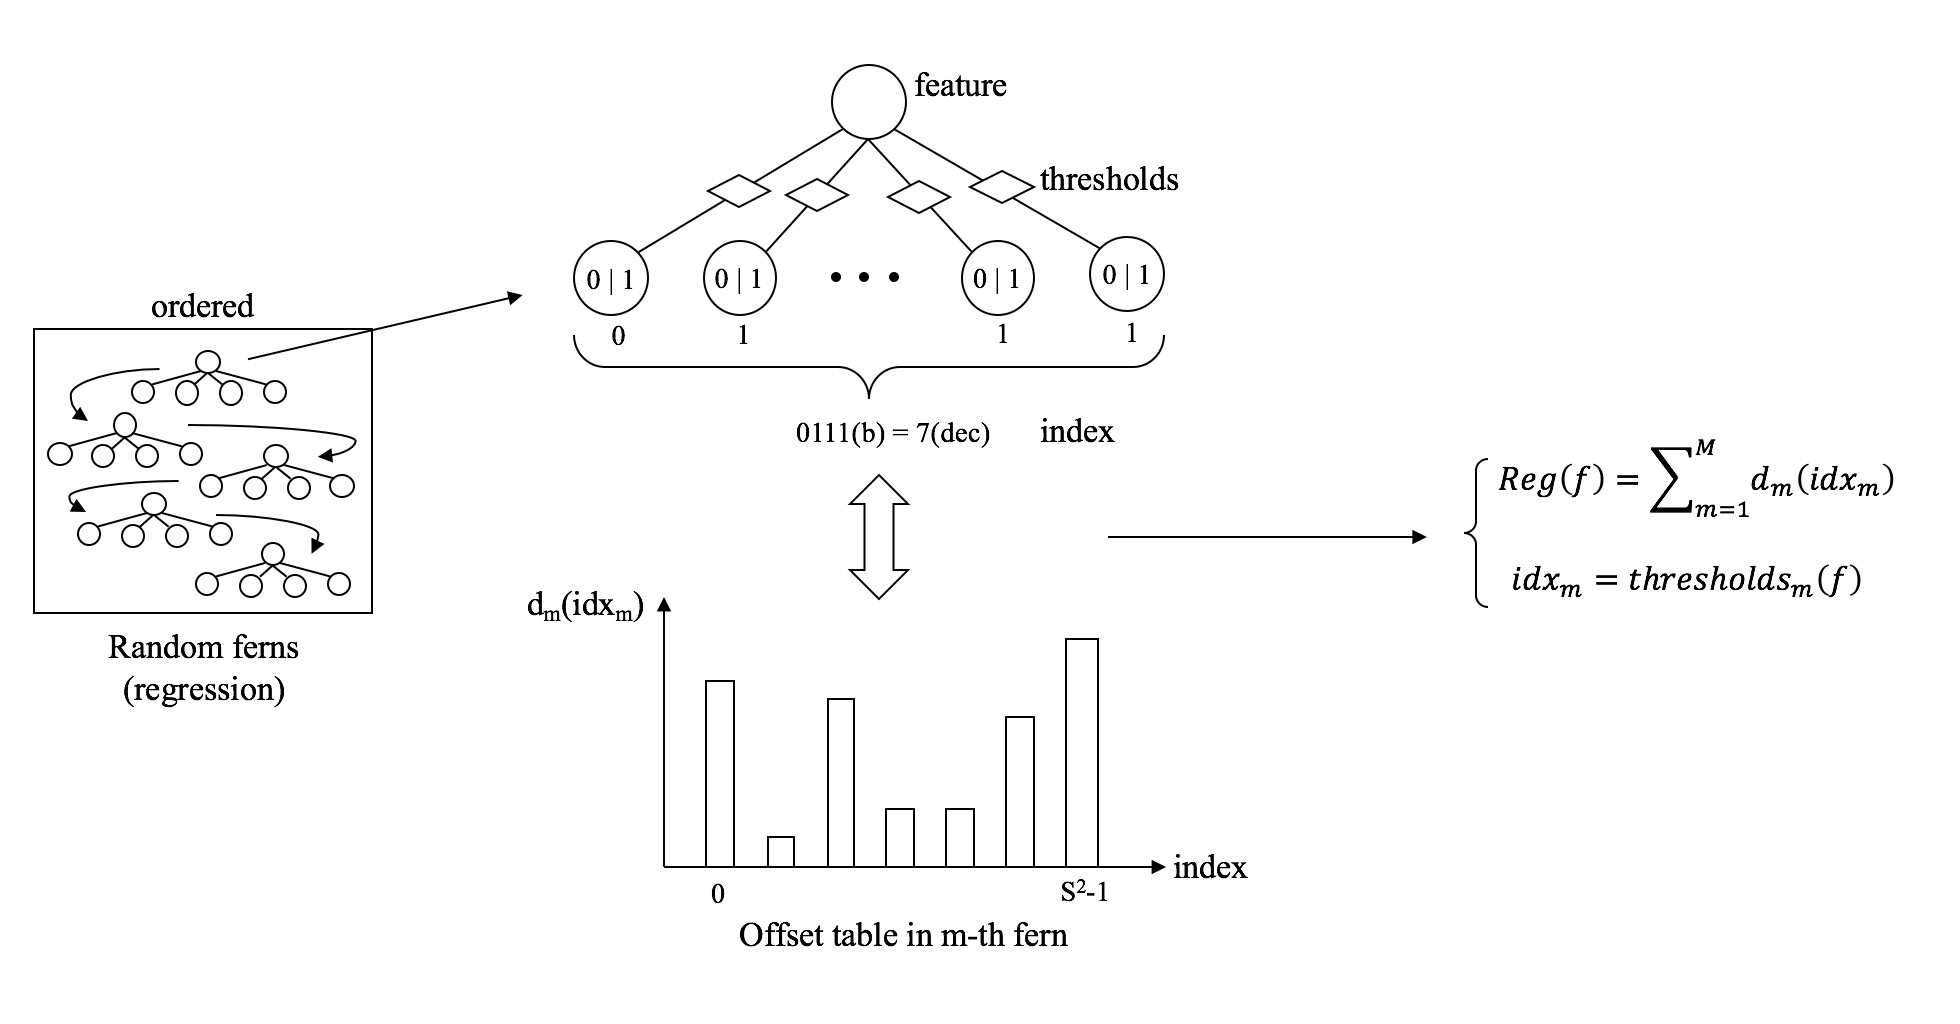
\includegraphics[width=\textwidth]{./mypic/改进后的随机蕨算法示意图.jpg} 
	\caption{改进后用于回归问题的随机蕨算法示意图} 
\end{figure}

上文表达了将随机蕨算法的核心思想,但是在实际实现该算法的时候仍将会遇到很多问题。过拟合问题是所有拟合算法中最常见的一种现象,这种现象也存在于随机蕨算法中。这一点可以通过在每一层基础蕨回归之后对每一层的回归量设置一个回归率,通过限制每一层的基础蕨的回归量上限可以非常好的抑制过拟合。虽然这种方法牺牲了一定的算法收敛速度,但是整体而言随机蕨回归算法仍旧有很高的计算速度。另外,在计算机代码实现过程中,随着随机蕨层数的增加,回归目标渐渐收敛,随机蕨的回归修正量会遇到浮点数的精度丢失问题。这个时候就需要利用额外记录每一层随机蕨回归目标均值作为保障。Algorithm 1 伪代码为随机蕨回归算法的整体概要。
% \newline
\newpage

\begin{algorithm}
\caption{随机蕨回归算法————训练模型 (Part I)}
\begin{algorithmic}[1]
\Require $D(data), L(label)$
\Require $S(depth), M(number\ of\ ferns), R(repeat\ times), eta(learning\ rate)$
\Ensure 随机蕨回归模型
\State 初始化:输入数据归一化等预处理;
\For{$M\ times$}
\Comment{随机蕨层数}
	\State $Loss_{min}\leftarrow MAX$
	\For{$R\ times$}
	\Comment{每层随机蕨重复随机过程次数}
		\State 随机产生S个维度与S个阈值:$dims, thresholds$
		\State $binary\ code=Compare(dims(D), thresholds)$
		\State \Comment 得到该基础蕨下所有训练样本的分类索引值
		\State 计算所有类内均值:$means$
		\State 更新所有训练样本的回归结果,计算$Loss$
		\If{$Loss<Loss_{min}$}
			\State 记录该基础蕨作为最佳基础蕨
% \algstore{bkbreak}
% \end{algorithmic}
% \end{algorithm}

% \begin{algorithm}
% \caption*{随机蕨回归算法————训练模型 (Part II)}
% \begin{algorithmic}[1]
% \algrestore{bkbreak}
			\State 保存该基础蕨的随机过程结果以及该随机过程下的训练样本分类均值
		\Else 
			\State $continue$
		\EndIf
	\EndFor
	\State $Y_{new}=Y_{original}-\sum_{i=0}^{m-1} Y_{pred_i}\cdot eta$
	\State \Comment 使用本次训练得到的最佳基础蕨的回归结果结合学习率更新回归目标
\EndFor
	% \State hh
\end{algorithmic}
\end{algorithm}


\begin{algorithm}
\caption{随机蕨回归算法————应用模型}
\begin{algorithmic}[1]
\Require $D(data)$,随机蕨回归模型
\Ensure $L(label)$
\State $Reg\leftarrow 0$
\Comment 初始化回归值
\For{$M\ times$}
\Comment{随机蕨层数}
	\State $binary\ code_m=Compare(dims_m(D), thresholds_m)$
	\Comment 得到本层基础随机蕨分类索引
	\State $reg_m=Indexing_m(binary\ code_m)$
	\Comment 得到本层基础随机蕨的回归值
	\State $Reg=Reg+reg_m$
	\Comment 将本次回归值累计到总回归值中去
\EndFor
\State \Return $Reg$
\end{algorithmic}
\end{algorithm}


% \newpage
% \pagebreak

\section{大噪声干扰下的随机蕨回归算法}

上一节中介绍了最基本的随机蕨回归模型,该模型在通常情况下都具有非常好的拟合能力,对于各种线性或者非线形问题都有很强的适应性。并且随机蕨回归算法在学习率的影响下,有非常好的抗过拟合能力,对轻微噪声也有很好的适应性。但是在实际应用过程中,会遇到一些数据极其不完备的情况。例如在一些回归问题中,输入的样本维度具有一定的不确定性,又或者在某些情况下输入样本的维度是一定的,但是有些维度的数据会存在严重噪声,如图2-3所示。

\begin{figure}[htb]
	\centering 
	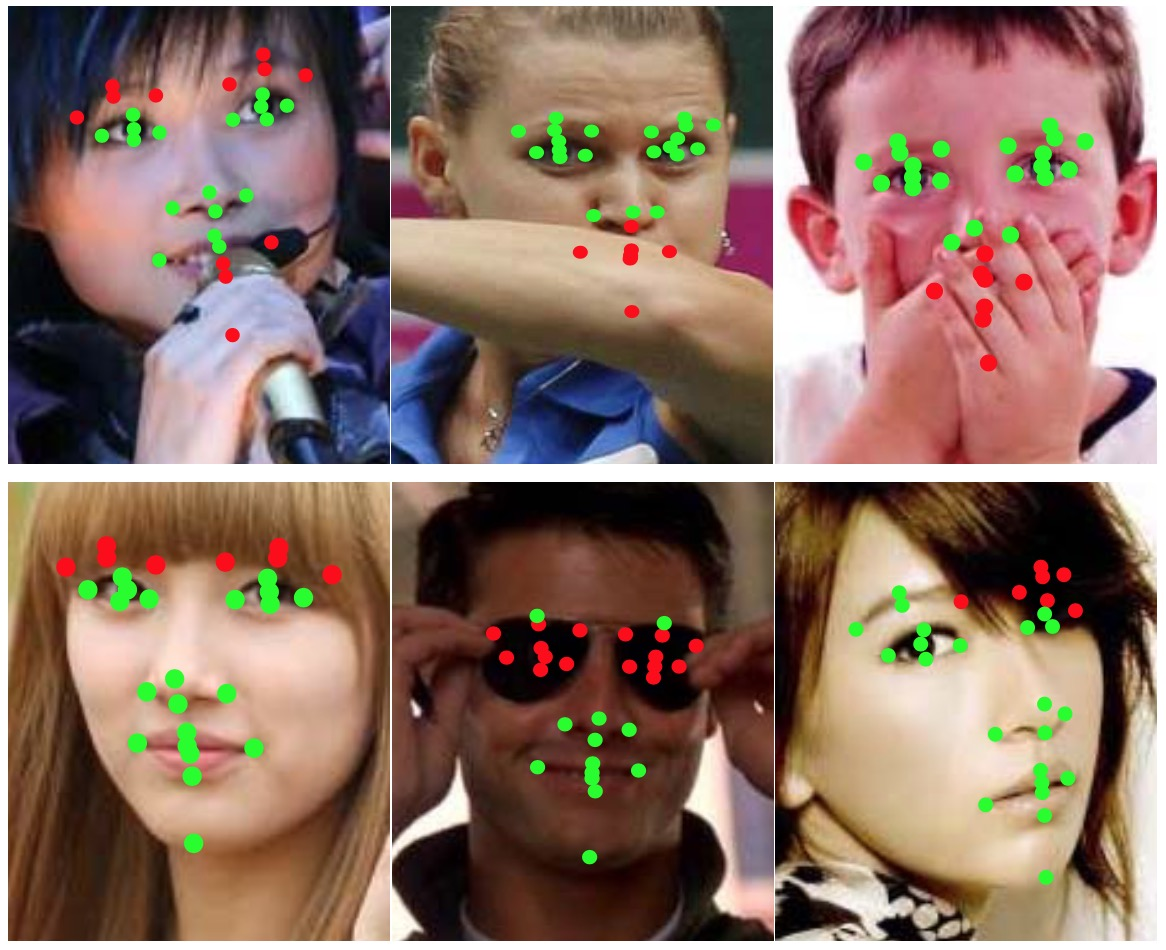
\includegraphics[width=0.7\textwidth]{./mypic/人脸特征由于被遮挡导致的缺失.jpg} 
	% 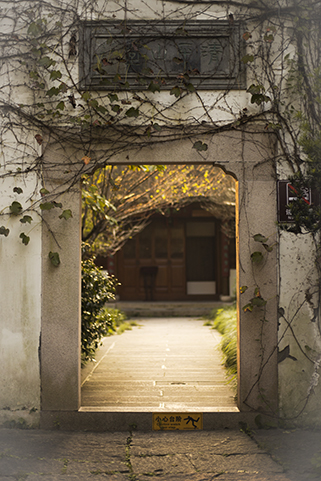
\includegraphics[scale=1.0]{./Pictures/test.jpg} 
	\caption{人脸特征(红点处)由于被障碍物遮挡导致缺失,缺失处的特征丧失了全部信息。} 
\end{figure}

这些情况下,在实验中会发现上节所述的随机蕨回归算法会遇到一个拟合能力严重不足的问题。例如存在一个输入样本特征描述$F=\{f_1,f_2,...,f_N\}$,其中有部分特征被噪声严重干扰,或者数据缺失,此时$F$为:
\begin{equation}
F=\{f_1,f_2,...f_p,f’_{p+1},...,f’_N\}
\end{equation}
其中$p+1$到$N$维特征为被噪声严重干扰的部分。这里注意随机蕨回归算法由于在选择特征维度的过程是完全随机的,不同样本也会有不同的被污染维度。例如在某一个样本中,前10个维度的特征被污染了,但是在另一个样本中后10个维度的特征被污染了,又或者在其他样本中完全随机的某些维度被污染。由于随机蕨算法中,每个基础蕨进行比较的那些维度($dims$)是完全随机生成的,因此为了方便后文阐述,上式中对于某一个样本,可以将被噪声严重污染的维度置于公式后方。

当特征存在上述被干扰情况的时候,从随机蕨算法中可以很容易看出,随机蕨算法存在两个缺陷。第一是当训练数据被干扰时,随机蕨回归模型在训练的过程中会尽量避免这些被污染的特征维度。因为一旦在随机过程中这些特征被选中,被污染的数据将会有错误的分类,并在最后分类均值的计算中严重干扰最后结果,最终导致整个随机蕨回归能力大大下降。第二是当随机蕨回归模型在训练的过程中并没有遇到严重的特征干扰问题,但是在实际应用过程中特征被大量污染以及干扰,这个时候被污染的特征维度直接导致样本的分类结果出现严重的偏差,就会导致最后的回归结果出现完全不在预期内的错误结果。

假设特征的被污染情况是可以被预测的(事实上在很多情况下这个假设是成立的,并且可以被很精确的估计),那么可以存在如下表达:
\begin{equation}
	B=\{b_1,b_2,...b_p,b_{p+1},...,b_N\}\in[0,1]
\end{equation}
其中$B$和$F$具有完全一致的维度,表示$F$的各个维度的置信度,也就是当$F$中某一维度的特征$F_i$被污染了的时候,对应的$B_i$将从百分之百可信度变为零(从1到0)。式(2-11)中假定第$1$到第$p$维都是未被污染的维度,第$p+1$到第$N$维都是被污染的维度,则有:
\begin{equation}
b_i=
\begin{cases}
1\quad {0\leq i\leq p} \\
0\quad {p<i\leq N}
\end{cases}
\end{equation}
$B$可以称为特征$F$的可信度掩码。在这个假设成立的情况下,我们可以充分利用这个信息来调整随机蕨回归算法。由于随机蕨算法中的每一个基础蕨都会根据出入特征的某几个维度进行回归,每个基础蕨在进行实际的回归之前可以先进行判断。如果该基础随机蕨要参考的那几个特征维度的可信度掩码值较低,则需要对这个随机蕨的回归量进行抑制,而当基础随机蕨参考的特征维度的可信度掩码值较高的时候,则对这个基础蕨的回归量不做调整。在算法实现过程中,特征维度的可信度掩码可以作为每个随机蕨的权值添加进算法中,也就是每个基础蕨的回归量应有如下表达:
\begin{equation}
	Reg_{fern}^{new} = Reg_{fern}^{original}\cdot f(B)
\end{equation}
其中$f(B)$为由可信度掩码生成的权值函数。在简单应用中,$f(B)$可以有简单的表达:
\begin{equation}
\begin{aligned}
	Q(i)=
	\begin{cases}
		1\quad i\in dims \\
		0\quad i\not\in dims
	\end{cases} \\
	f(B)=\frac{\sum_{i\in dims} b_i}{\sum_{i=0}^{N} Q(i)}
\end{aligned}
\end{equation}
在有了权值调整之后,当某一个基础蕨进行特征维度和阈值的比较时,会同时对可信度掩码进行处理。一旦输入的样本特征有较低的可行度时,$f(B)$将得到一个较低的值,从而抑制住这个基础蕨的回归量,避免杂乱的回归量对最后结果有较大的影响。并且这样处理仍然能让所有的维度都得到均匀的训练,不然被污染的维度会由于训练时$Loss$下降过少而被训练器忽略。同时在回归应用的时候,被污染的特征维度也会被抑制,保证最后回归结果不会因为某几个特征维度的干扰而破坏。

Algorithm 3 为增加掩码了机制的随机蕨算法的伪代码。
% \newline

\begin{algorithm}
\caption{掩码机制下的随机蕨回归算法————训练模型}
\begin{algorithmic}[1]
\Require $D(data), L(label), B(belief\ mask)$
\Require $S(depth), M(number\ of\ ferns), R(repeat\ times), eta(learning\ rate)$
\Ensure 随机蕨回归模型
\State 初始化:输入数据归一化等预处理;
\For{$M\ times$}
\Comment{随机蕨层数}
	\State $Loss_{min}\leftarrow MAX$
	\For{$R\ times$}
	\Comment{每层随机蕨重复随机过程次数}
		\State 随机产生S个维度与S个阈值:$dims, thresholds$
		\State $binary\ code=Compare(dims(D), thresholds)$
		\State \Comment 得到该基础蕨下所有训练样本的分类索引值
		\State $f(B)=\frac{\sum_{i\in dims} b_i}{\sum_{i=0}^{N} Q(i)}$
		\State \Comment 根据该基础蕨所选特征的置信度计算该基础蕨的回归量权值
		\State 计算所有类内均值:$means$
		\State $Y_{pred_i}=means(binary\ code)$
		\State $Y_{new}=Y_{original}-f(B)\cdot \sum_{i=0}^{m-1} Y_{pred_i}\cdot eta$
		\State \Comment 使用本次训练得到的基础蕨的回归结果结合学习率以及权值更新回归目标
		\State $Loss=\sum_i{\|Y_{new,i}-\overline{L_i}\|}$
		\State \Comment 计算$Loss$
		\If{$Loss<Loss_{min}$}
			\State 记录该基础蕨作为最佳基础蕨
			\State 保存该基础蕨的随机过程结果以及该随机过程下的训练样本分类均值
		\Else 
			\State $continue$
		\EndIf
	\State $\hat{Y}_{new}=\hat{Y}_{original}-\hat{f}(B)\cdot \sum_{i=0}^{m-1} \hat{Y}_{pred_i}\cdot eta$
	\State \Comment 使用最佳基础蕨的回归结果结合学习率以及权值更新回归目标
	\EndFor
\EndFor
\end{algorithmic}
\end{algorithm}

\begin{algorithm}
\caption{掩码机制下的随机蕨回归算法————应用模型}
\begin{algorithmic}[1]
\Require $D(data), B(belief\ mask)$,随机蕨回归模型
\Ensure $L(label)$
\State $Reg\leftarrow 0$
\Comment 初始化回归值
\For{$M\ times$}
\Comment{随机蕨层数}
	\State $binary\ code_m=Compare(dims_m(D), thresholds_m)$
	\Comment 得到本层基础随机蕨分类索引
	\State $reg_m=Indexing_m(binary\ code_m)$
	\Comment 得到本层基础随机蕨的回归值
	\State $Reg=Reg+reg_m$
	\Comment 将本次回归值累计到总回归值中去
\EndFor
\State \Return $Reg$
\end{algorithmic}
\end{algorithm}


\newpage

\section{实验结果与分析} % 人脸回归可以在这里写

为了验证随机蕨算法从分类问题下改进到回归问题下的合理性,本文进行了两个步骤的验证实验。首先通过一个基础拟合问题验证其基本的拟合能力,特别是对于非线性问题的拟合能力。然后在将其应用到人脸特征点定位这个高纬度、非线性的实际问题中,进一步验证其回归能力的鲁棒性。

% \subsection{对随机蕨拟合能力的验证} %

首先验证随机蕨回归算法对于非线形问题的拟合能力,本文通过构造几个非线性函数,并添加随机噪声作为测试数据进行检验。

非线性函数具有如下表达式:
\begin{equation}
	f(x) = \cos(\lambda_1\pi x)+ \lambda_2 (x+1)^2 + \lambda_3 log(x+1) + \lambda_4
\end{equation}
其中包含三角函数项、多项式函数项、以及指数性质项,每给定任意的一组$\lambda_i$参数就可以得到一个特定的非线性函数。为了定量衡量算法回归能力,本文基于上述非线性函数,在自变量区间为$[0,1]$之间随机采样500个点,同时为函数值附加方差为$\sigma^2$的高斯噪声作为拟合模型的训练数据。最后将得到的拟合模型与原始函数进行比对,在同样自变量区间取1000个采样点,计算其与真值的方差$\hat{\sigma}^2$,以方差减少量作为拟合效果的评价指标。

表格2-1给出了其中20次随机实验的结果。实验中用于随机蕨拟合回归的训练参数为:学习率$eta=0.02$,$S=4$,$M=150$,$R=20$。从实验结果可以看出,原本存在较大方差噪声的数据经过随机蕨拟合回归之后,与原始模型相比方差减少幅度均值在95\%左右,对于非线性问题具有非常好的拟合能力。

图2-4给出了一些可视化数据。图中蓝色点表示用于训练随机蕨回归模型的训练数据点,红色点为随机蕨回归模型训练好之后预测的原始函数,绿色点表示原始函数真值。可以看到,图中红色点与绿色点已经非常接近,表明了随机蕨算法的拟合能力得到了验证。

\begin{table}[htb]
	\zihao{5}
	\caption{随机蕨拟合能力检验结果表} 
	% \label{Tabkeyword}
	\centering 
	\begin{tabular}[t]{
		% |c|l|r|p{4cm}|} 
		ccccccc} 
		\toprule
		$\lambda_1$ & $\lambda_2$ & $\lambda_3$ & $\lambda_4$ & 噪声方差 & 拟合后方差 & 方差减少幅度\\ 
		\midrule
		3.37292 & 0.649499 & 0.649499 & 0.649499 & 0.5 &    0.0124&    97.5229\% \\
		3.53833 & 0.792932 & 0.792932 & 0.792932 & 0.5 &    0.0153&    96.9383\% \\
		2.99967 & -0.525472 & -0.525472 & -0.525472 & 0.5 &    0.0119&    97.6265\% \\
		2.575 & 1.9678 & 1.9678 & 1.9678 & 0.5 &    0.0070&    98.6014\% \\
		2.15032 & 0.461065 & 0.461065 & 0.461065 & 0.5 &    0.0148&    97.0353\% \\
		3.09489 & -0.157773 & -0.157773 & -0.157773 & 0.5 &    0.0080&    98.3986\% \\
		5.09176 & 1.26823 & 1.26823 & 1.26823 & 0.5 &    0.0293 &    94.1431\% \\
		3.61479 & 1.71666 & 1.71666 & 1.71666 & 0.5 &    0.0133&    97.3352\% \\
		2.66396 & 1.1875 & 1.1875 & 1.1875 & 0.5 &    0.0102&    97.9562\% \\
		3.29159 & 1.72562 & 1.72562 & 1.72562 & 0.5 &    0.0160&    96.7915\% \\
		4.97152 & 0.308569 & 0.308569 & 0.308569 & 0.5 &    0.0430&    91.3997\% \\
		3.38681 & -1.90669 & -1.90669 & -1.90669 & 0.5 &    0.0102&    97.9517\% \\
		3.80523 & -1.54795 & -1.54795 & -1.54795 & 0.5 &    0.0108&    97.8402\% \\
		5.27595 & 0.855638 & 0.855638 & 0.855638 & 0.5 &    0.0287 &    94.2662\% \\
		2.22052 & 0.2368 & 0.2368 & 0.2368 & 0.5 &    0.0064&    98.7156\% \\
		5.79584 & -1.26993 & -1.26993 & -1.26993 & 0.5 &    0.0483&    90.3486\% \\
		2.42347 & -0.731821 & -0.731821 & -0.731821 & 0.5 &    0.0113&    97.7331\% \\
		4.42034 & 0.694184 & 0.694184 & 0.694184 & 0.5 &    0.0131&    97.3814\% \\
		4.83876 & 1.05292 & 1.05292 & 1.05292 & 0.5 &    0.0305&    93.8946\% \\
		\bottomrule
	\end{tabular}
\end{table}


\begin{figure}[htb]
	\centering 
	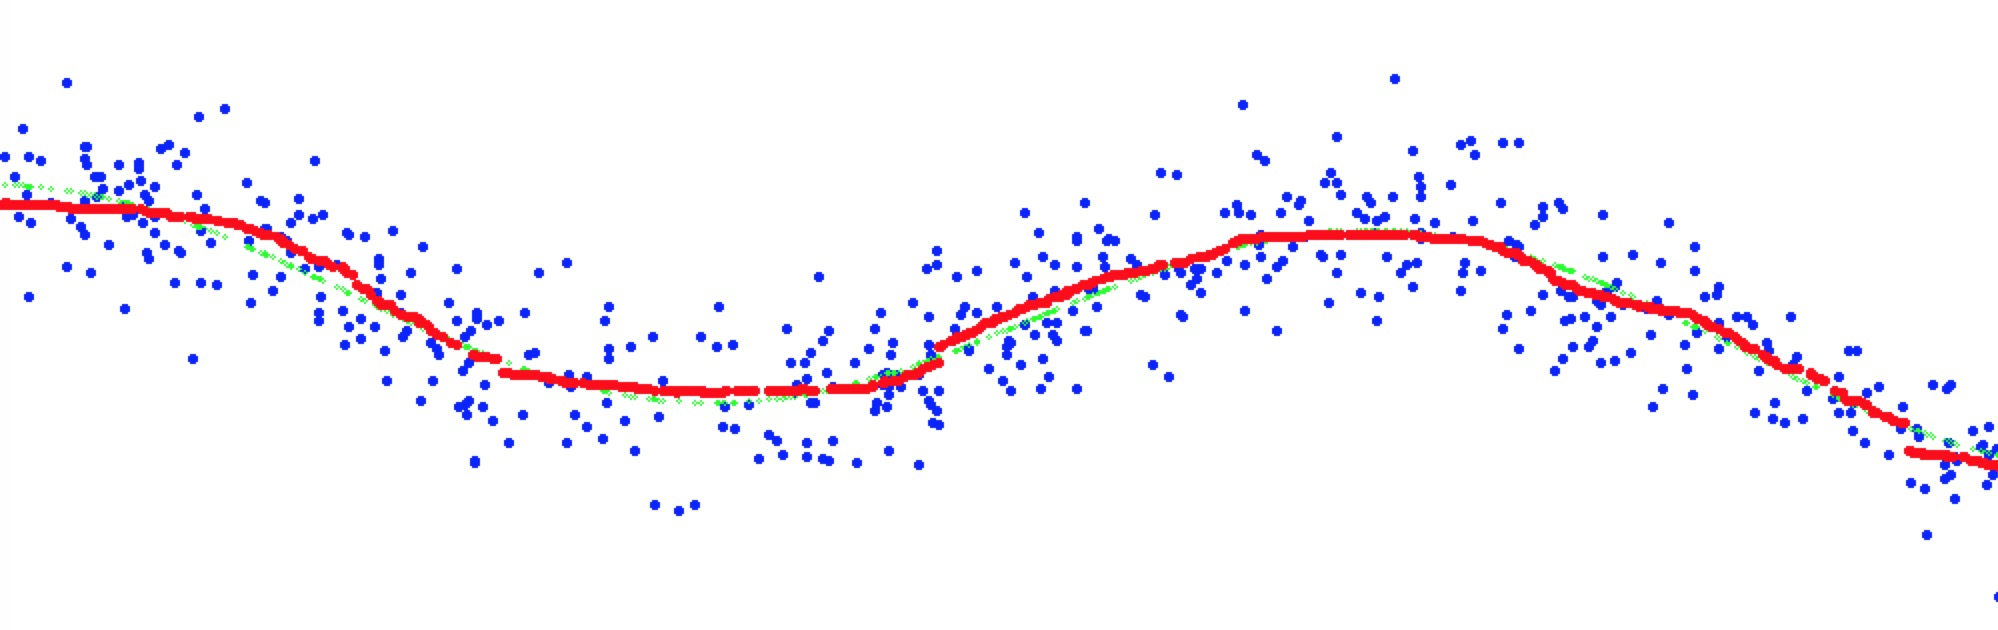
\includegraphics[width=0.6\textwidth]{./mypic/随机蕨回归实验1.jpg} 
	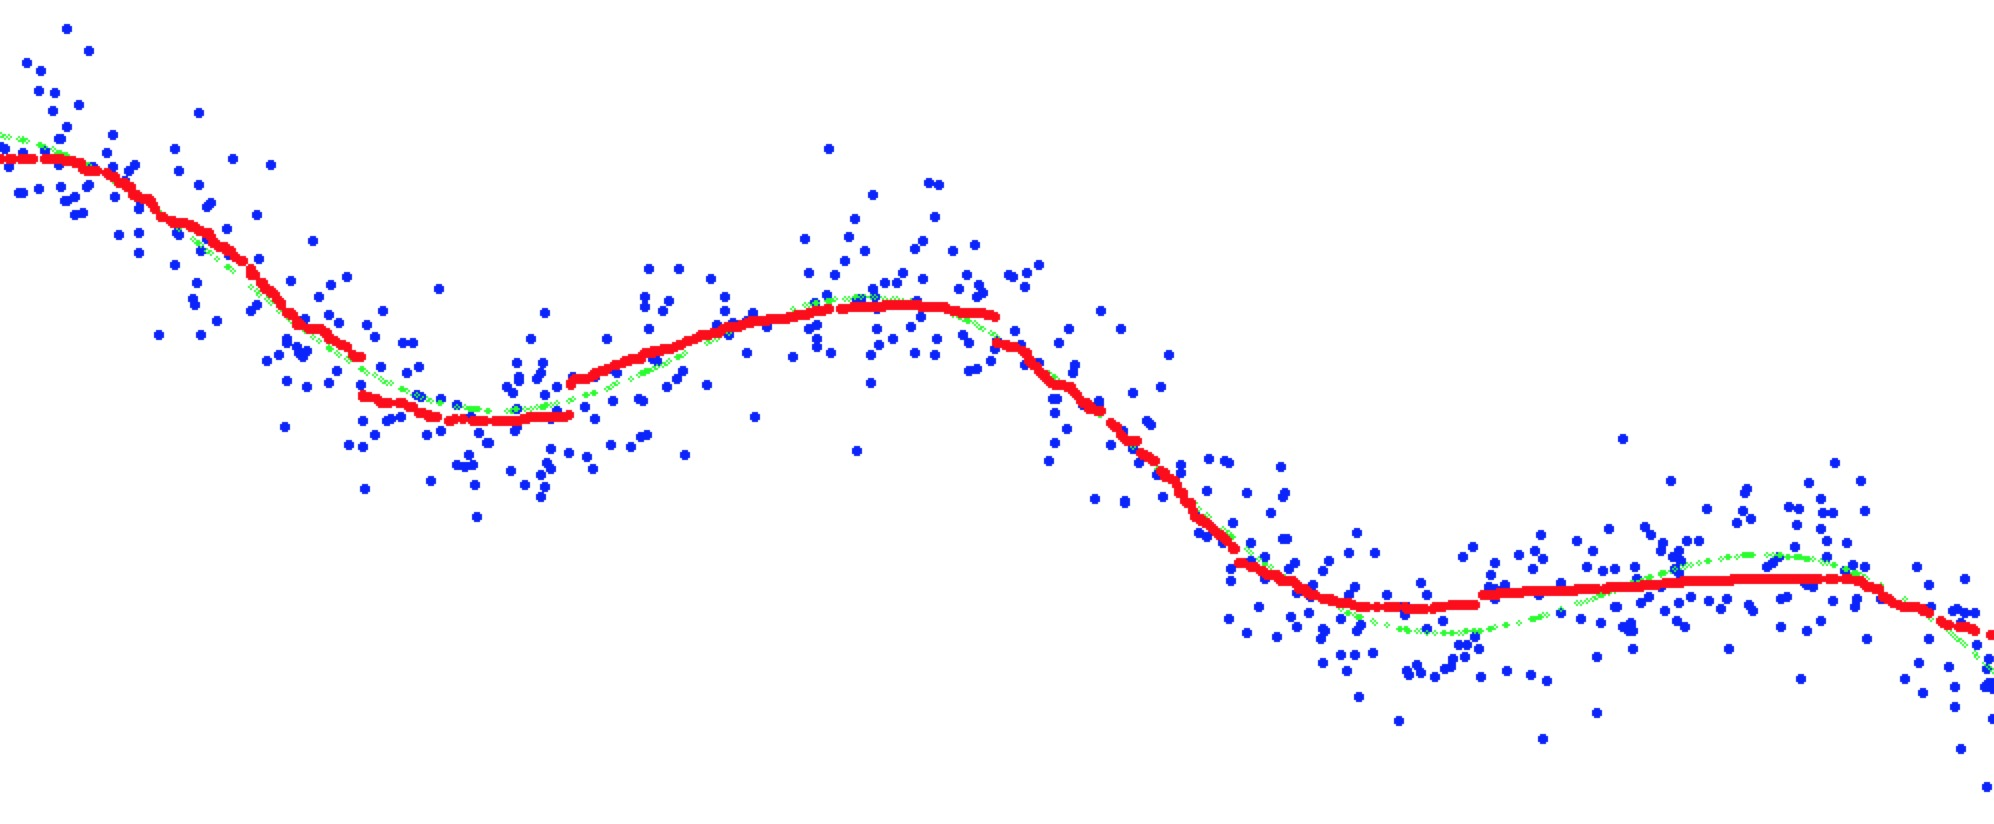
\includegraphics[width=0.6\textwidth]{./mypic/随机蕨回归实验2.jpg} 
	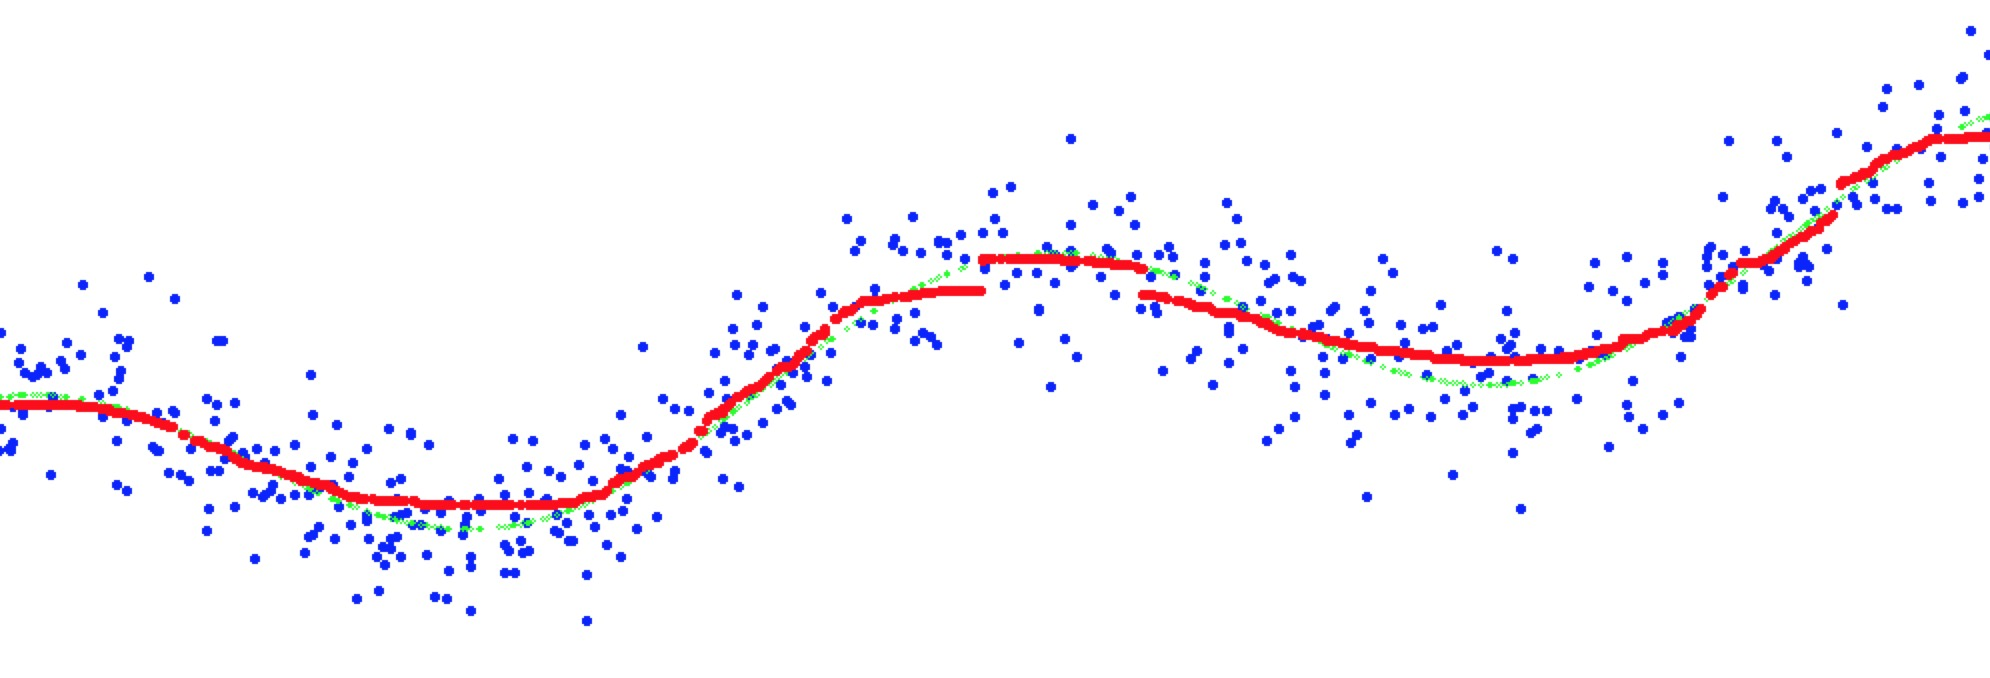
\includegraphics[width=0.6\textwidth]{./mypic/随机蕨回归实验3.jpg} 
	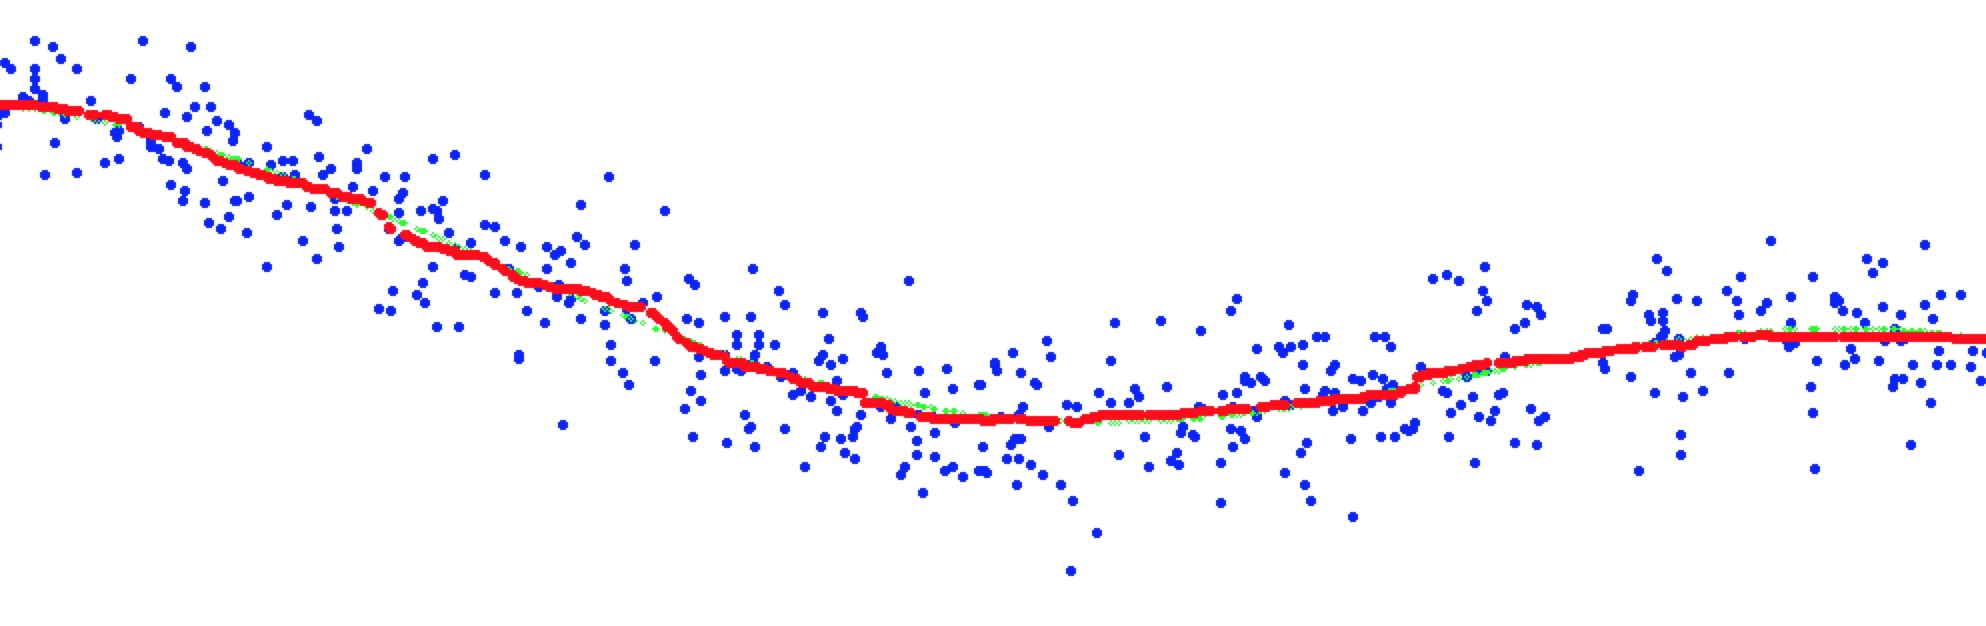
\includegraphics[width=0.6\textwidth]{./mypic/随机蕨回归实验4.jpg} 
	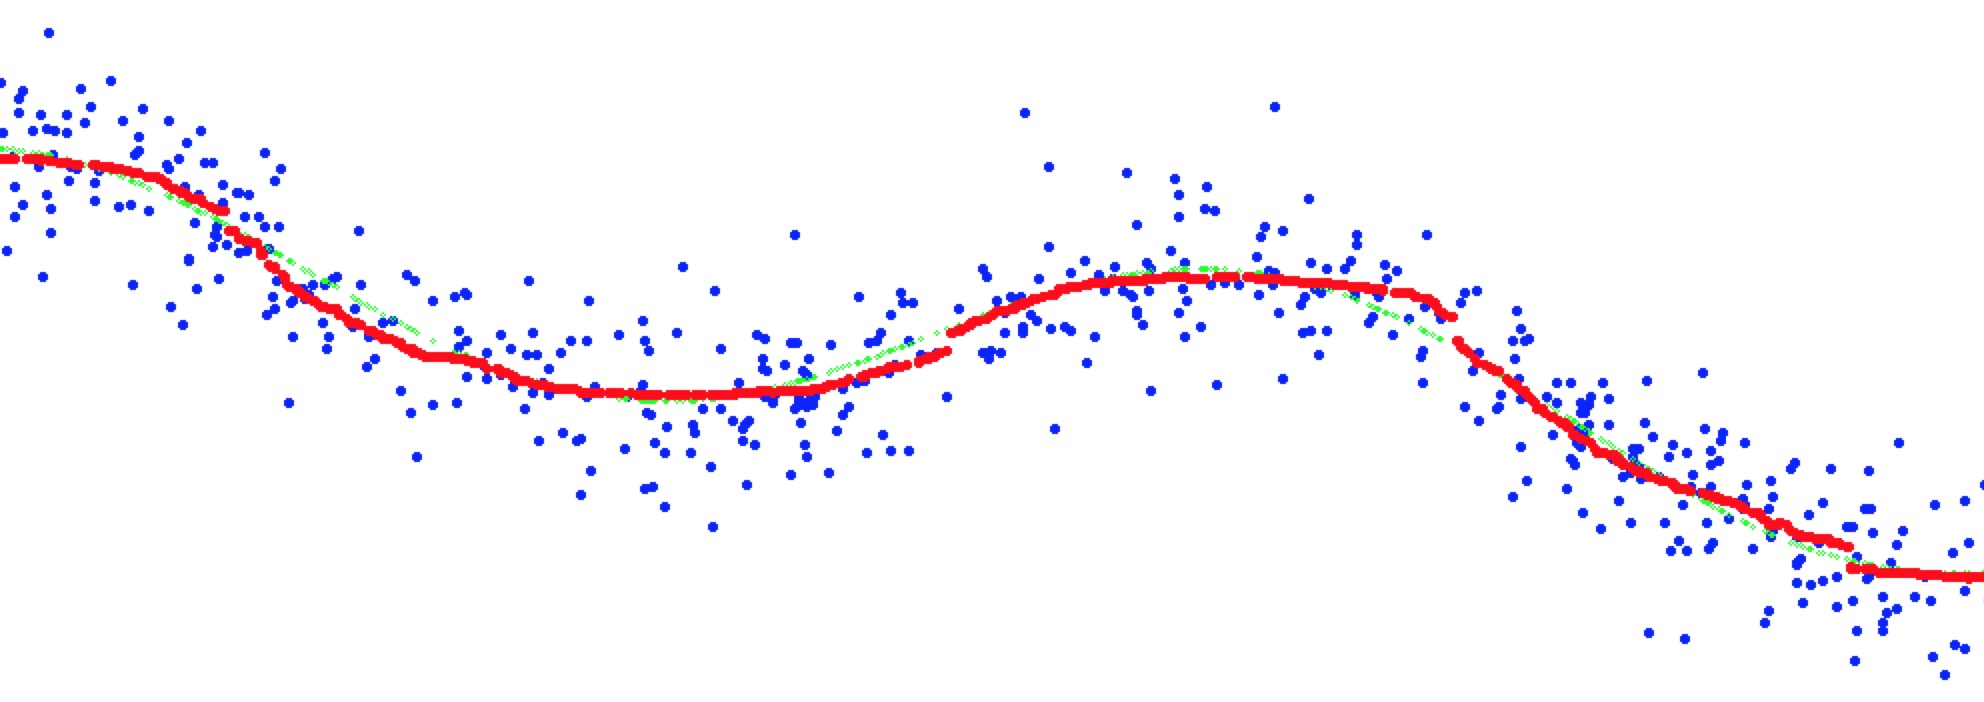
\includegraphics[width=0.6\textwidth]{./mypic/随机蕨回归实验5.jpg} 
	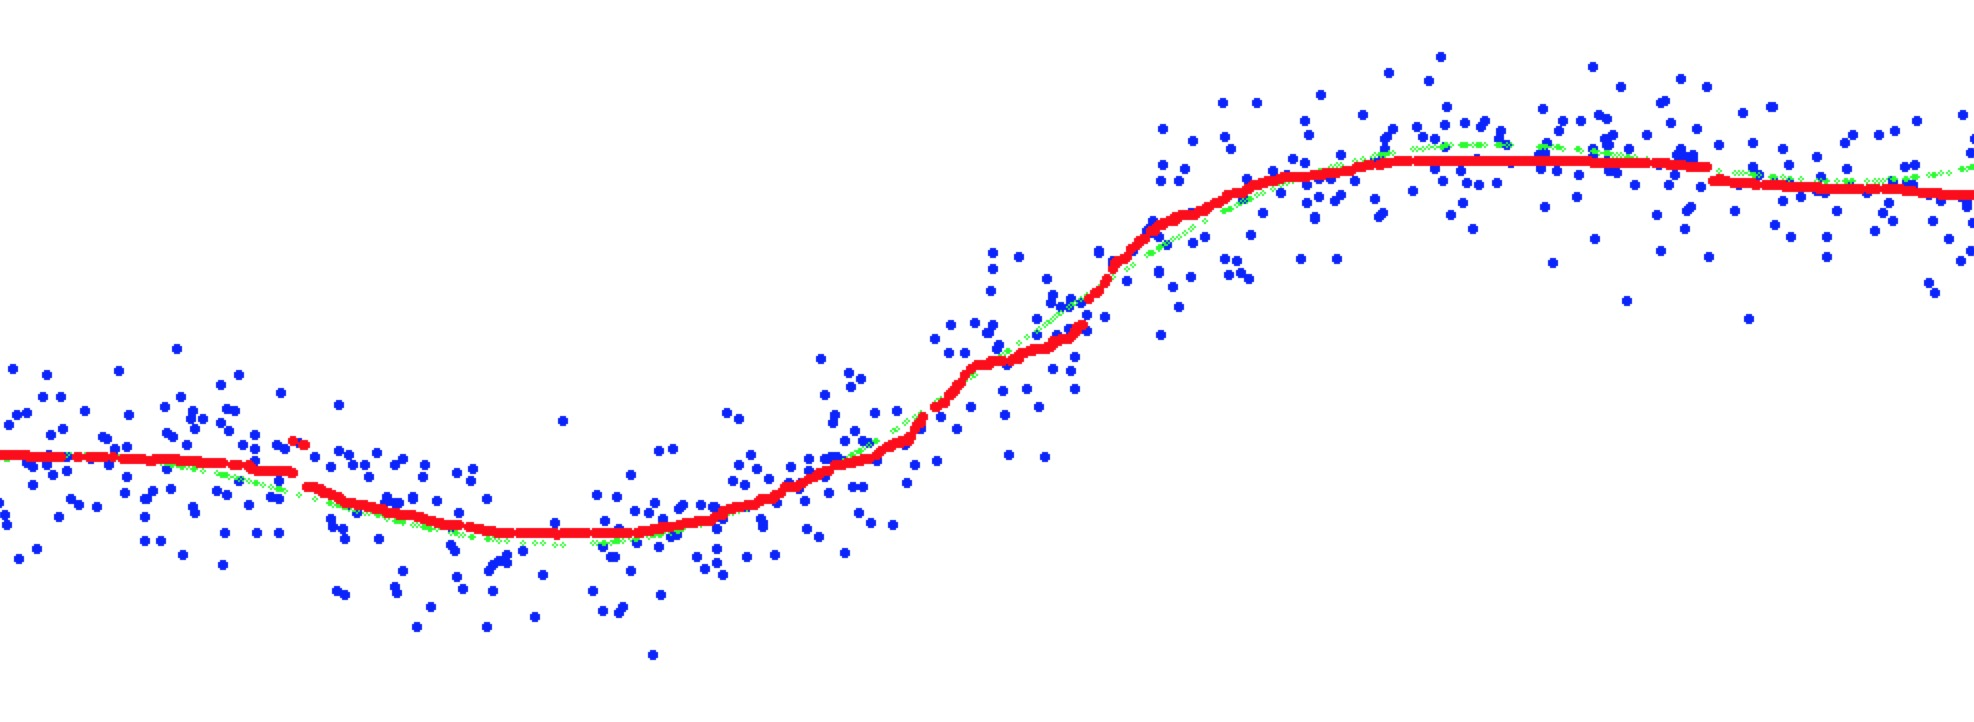
\includegraphics[width=0.6\textwidth]{./mypic/随机蕨回归实验6.jpg} 
	% 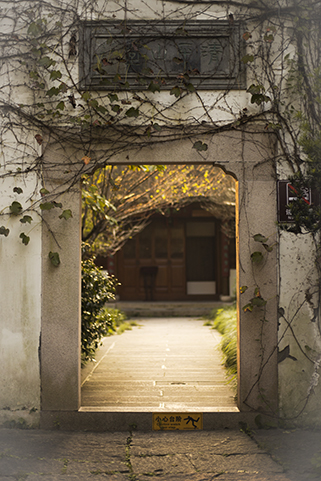
\includegraphics[scale=1.0]{./Pictures/test.jpg} 
	\caption{随机蕨回归实验可视化结果} 
\end{figure}

除此之外,本文还将该随机蕨回归算法应用到人脸特征点定位这个更为复杂的回归问题中去,同样也取得了非常不错的表现。由于该实验涉及一些与本文相关度不高的中间步骤,因此具体实验细节在此不作详述,仅给出实验最后得到的人脸特征点定位结果。图2-5中红色圆点表示通过随机蕨回归器得到的人脸特征点定位结果。该实验中涉及的随机蕨回归模型具有高达1000维度输入以及136维度的回归目标,具有极高的回归复杂度。其优良的表现再次证明了随机蕨回归算法的可行性。

并且,本文将该人脸特征点定位算法结果与现有最为优秀的几个算法进行了比较。通过在300-W数据集\cite{sagonas2013semi}上,采用瞳孔间距正则化误差作为评价标准\cite{belhumeur2013localizing}\cite{cao2014face},本文得到如表2-2所示的结果。从表2-2可以看出,本文算法相比于ESR\cite{cao2014face}、SDM\cite{xiong2013supervised}、LBF fast\cite{ren2014face}这三种算法有更小的误差(其中300-W数据集包含一般数据集和复杂数据集两个部分),并且在算法效率上仅次于LBF fast。此实验中其他三种算法的实验结果均引用于文章[\citenum{ren2014face}],对于精度对比没有影响,但本文算法的帧率测试由于实验平台不同,仅供参考(本文实验环境为2.2GHz Intel Core i7单进程处理器)。该实验可以表明,改进后的随机蕨算法不光具有较好的拟合能力,同时也具备较高的计算效率。

\begin{figure}[htb]
	\centering 
	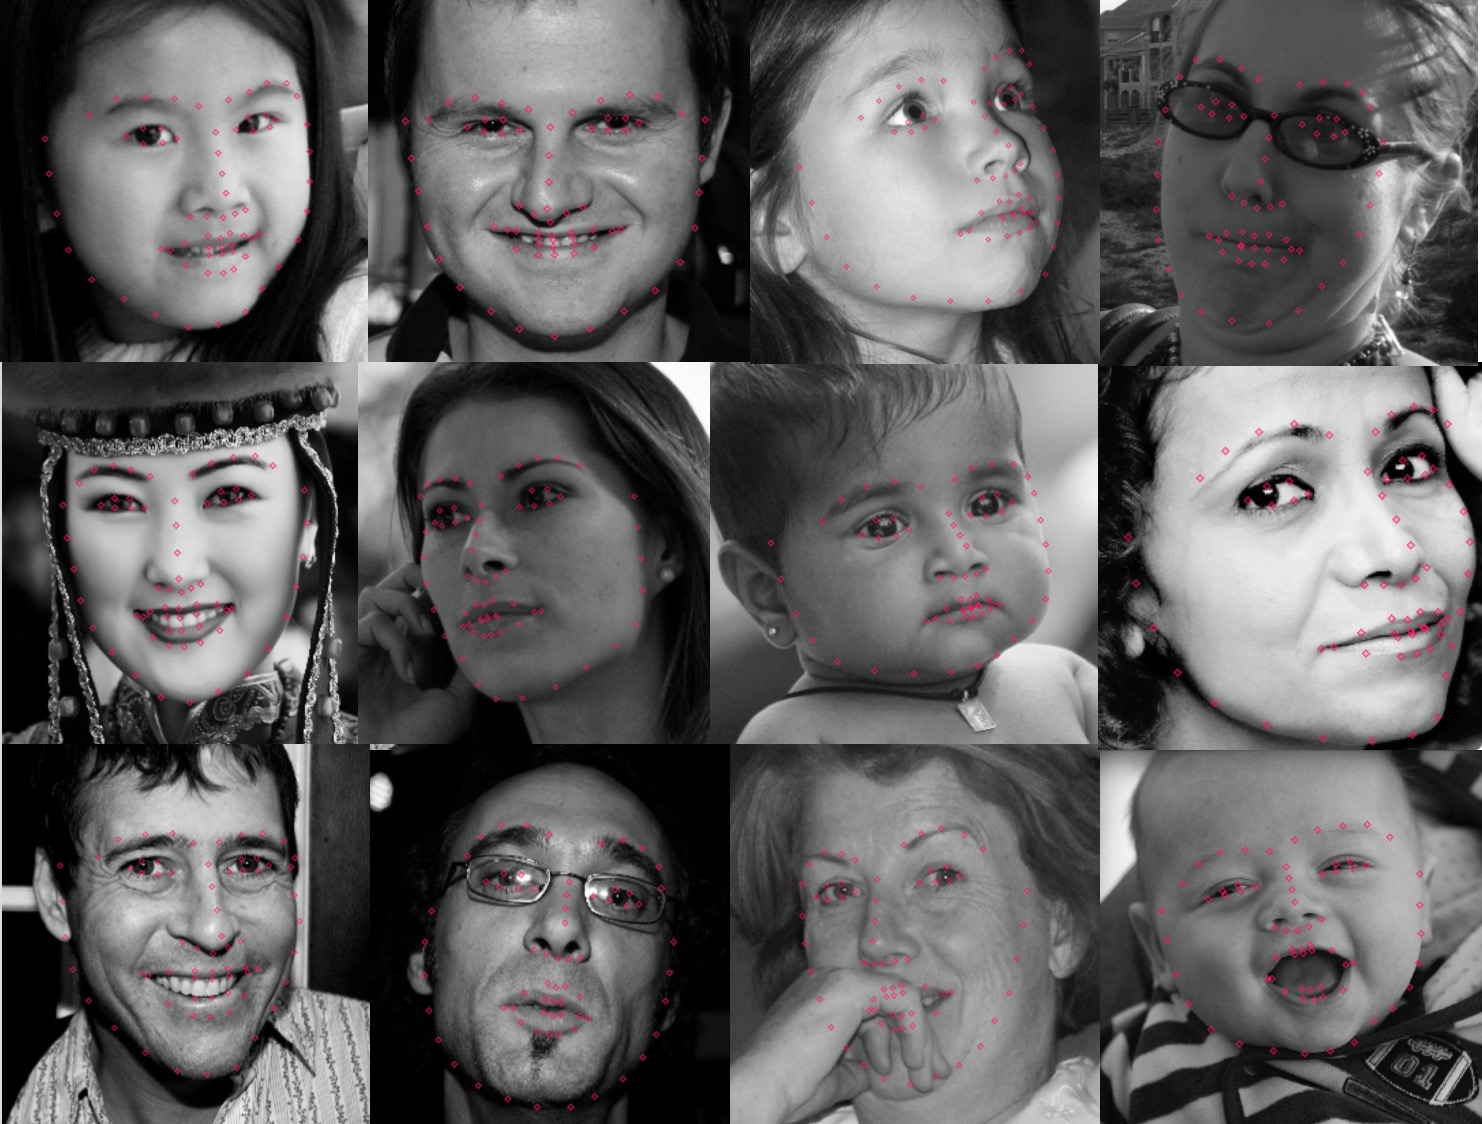
\includegraphics[width=\textwidth]{./mypic/人脸特征点定位实验.jpg} 
	% 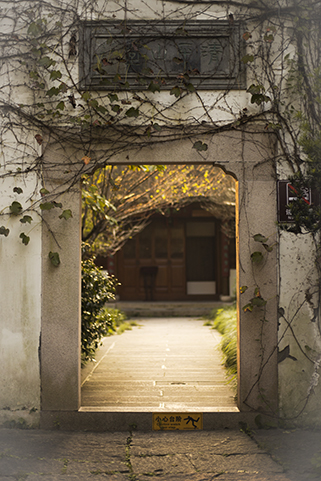
\includegraphics[scale=1.0]{./Pictures/test.jpg} 
	\caption{人脸特征点定位实验结果} 
\end{figure}

\begin{table}[htb]
	\zihao{5}
	\caption{300-W数据集上人脸特征点定位算法对比} 
	% \label{Tabkeyword}
	\centering 
	\begin{tabular}[t]{
		% |c|l|r|p{4cm}|} 
		ccccccc} 
		\toprule
		算法 & 全数据集误差 & 一般数据集误差 & 复杂数据集误差 & 帧率(FPS)\\ 
		\midrule
		ESR\cite{cao2014face} & 7.58 & 5.28 & 17.00 & 120 \\
		SDM\cite{xiong2013supervised} & 7.52 & 5.6 & 15.4 & 70 \\
		LBF fast\cite{ren2014face} & 7.37 & 5.38 & 15.5 & 3100 \\
		Ours & 6.94 & 4.93 & 15.18 & 476 \\
		\bottomrule
	\end{tabular}
\end{table}


% \subsection{对大噪声干扰下的随机蕨算法验证} % 

大噪声干扰下的随机蕨算法验证实验由于与本文第四章实验有较多相互依赖的交集,因此对于该问题的实验验证将在节4.6中进行展开,此处不再详细讨论。


\section{本章小结}
本章旨在充分开发随机蕨算法的潜能,通过改造整理,先是总结出经典随机蕨算法应用于回归问题的改进方法,再进一步结合实际问题中存在大噪声干扰下随机蕨算法不够鲁棒的情况,提出掩码机制下的随机蕨回归算法。最后还通过实验验证了随机蕨算法在非线性回归问题下的拟合能力,通过人脸特征点定位这个具有非常大挑战性的回归问题,证实了本章提出的随机蕨回归算法具有较好的实用性以及高效性。

























\chapter{test}

本章主要介绍仿真环境的搭建

\section{仿真环境搭建}

\begin{equation}
\begin{pmatrix} 
3 & 4 & 5 \\
0 & 1 & 2 \\
9 & 8 & 7  
\end{pmatrix}=
\begin{bmatrix} 
x_1 & x_2 & x_3 \\
y_1 & y_2 & y_3 \\
z_1 & z_2 & z_3 
\end{bmatrix} 
\end{equation}

\begin{lstlisting}[language={[ANSI]C}] 
int main(int argc, char ** argv) 
{ 
printf("Hello world! \n"); 
return 0; 
} 
\end{lstlisting}

\begin{algorithm}
\caption{A test algorithm (Part I)}
\begin{algorithmic}[1]
\Require <hahdsfasdfadf>
\Ensure <hahdsfasdfadf>
\State <hahdsfasdfadf>
\If{<condition>}
	\State <hahdsfasdfadf>
\ElsIf{<condition>}
	\State <hahdsfasdfadf>
\Else 
	\State <hahdsfasdfadf>
\EndIf
\For{<condition>}
	\State <hahdsfasdfadf>
\EndFor
\ForAll{<condition>}
	\State <hahdsfasdfadf>
\EndFor
\While{<condition>}
	\State <hahdsfasdfadf>
\EndWhile
\Repeat
	\State <hahdsfasdfadf>
\Until{<condition>}
\Loop
	\State <hahdsfasdfadf>
\EndLoop
    \algstore{bkbreak}
\end{algorithmic}
\end{algorithm}

\begin{algorithm}
\caption*{A test algorithm (Part II)}
\begin{algorithmic}[1]
\algrestore{bkbreak}
\Function{<name>}{<params>} <body> \EndFunction
\State \Return <hahdsfasdfadf>
\Comment{<comment>}
\Procedure {BellmanKalaba}{$G$, $u$, $l$, $p$}
\ForAll {$v \in V(G)$}
\State $l(v) \leftarrow \infty$
\EndFor
\State $p(i) \leftarrow v_j$
\State $l’(i) \leftarrow min$
\State $changed \leftarrow l \not= l’$
\EndProcedure
\end{algorithmic}
\end{algorithm}

% \begin{algorithm}[H]
% \caption{How to write algorithms}
% \KwIn{this text}
% \KwOut{how to write algorithm with \LaTeX2e }
% initialization\;
% \While{not at end of this document}{
%     read current\;
%     \eIf{understand}{
%         go to next section\;
%         current section becomes this one\;
%     }{
%         go back to the beginning of current section\;
%     }
% }
% \end{algorithm}

空行:
\newline

随机蕨最早由他[\citenum{ozuysal2007fast}]提出\cite{ozuysal2007fast}。

项目:\\
无序:
\begin{itemize}
\item[-] good morning...
\item[-] good morning....
\end{itemize}

\begin{itemize}
\item good evening...
\item good evening....
\end{itemize}

有序:
\begin{enumerate}
\item good morning...
\item good morning....
\end{enumerate}

公式:
\begin{equation}
	a^2=b^2+c^2+d^2
\end{equation}

行内公式:
balabala
$P(C_k|F)$
balabala

% Listing~\ref{lst:}

\begin{equation}
	OK
\end{equation}

图像:
\begin{figure}[htb]
	\centering 
	% 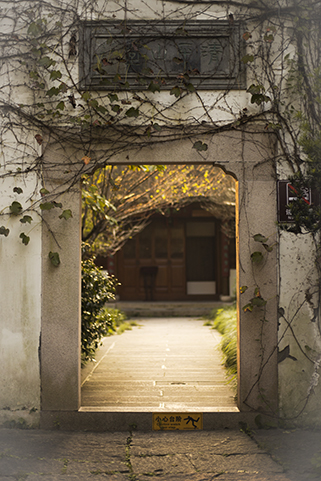
\includegraphics[width=\textwidth]{./Pictures/test.jpg} 
	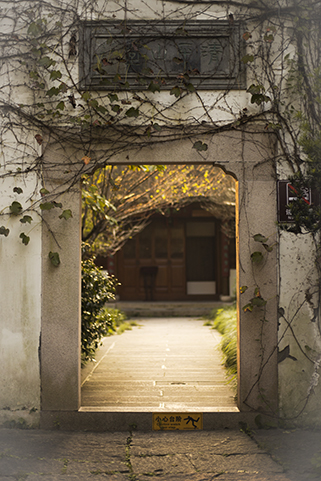
\includegraphics[scale=1.0]{./Pictures/test.jpg} 
	\caption{ljzst} 
\end{figure}

\begin{figure}[htb]
	\centering 
	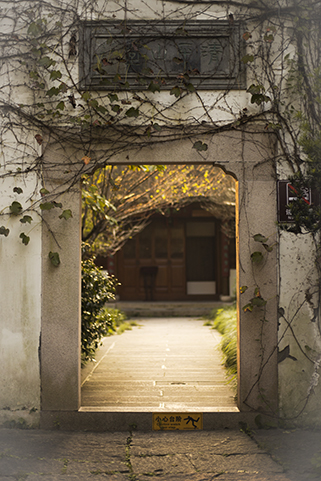
\includegraphics[width=\textwidth]{./Pictures/test.jpg} 
	% 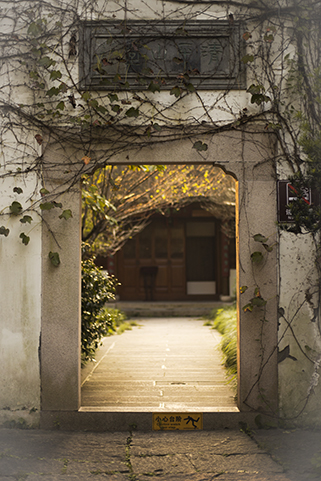
\includegraphics[scale=1.0]{./Pictures/test.jpg} 
	\caption{another way} 
\end{figure}

\begin{figure}[htb]
	\subfigure[img1]{ 
		\begin{minipage}[b]{0.5\textwidth} 
		\centering
		% \label{fig:SubFigure1} %% label for second subfigure 
		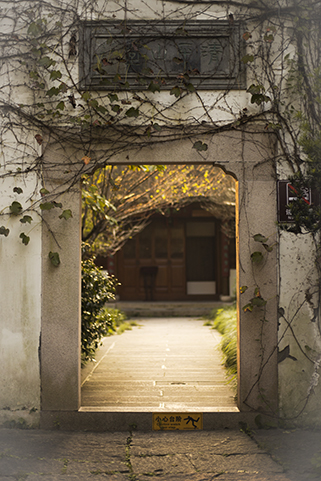
\includegraphics[scale=1.0]{./Pictures/test.jpg} 
		\end{minipage}}
	\subfigure[img2]{ 
		\begin{minipage}[b]{0.5\textwidth} 
		\centering
		% \label{fig:SubFigure1} %% label for second subfigure 
		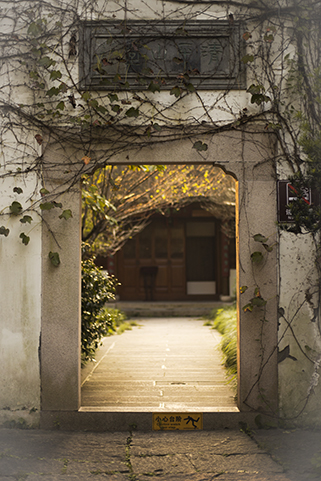
\includegraphics[scale=1.0]{./Pictures/test.jpg} 
		\end{minipage}}
	\caption{img all}
\end{figure}

{
\begin{table}[htb]
	\zihao{5}
	\caption{standard table} 
	% \label{Tabkeyword}
	\centering 
	\begin{tabular}[t]{
		|c|l|r|p{4cm}|} 
		\hline
		center & left & right & 靠左,并宽4cm\\ 
		\hline
		Center & Left & Right & Width=4cm\\ 
		\hline
	\end{tabular}
\end{table}
}

{
\begin{table}[htp]
	\zihao{5}
	\caption{复杂表格示例}
	% \label{TabComplex}
	\centering
	\begin{tabular}[t]{|c|c|c|c|c|}
		\hline
		\multicolumn{2}{|c|}{我占了两列} & 第3列 & 第4列 & 第5列\\
		\hline
		\multirow{2}*{我占了两行} & 第二行第2列 & 第二行第3列 & \multicolumn{2}{|c|}{\multirow{2}*{我占了两行又两列}}\\
		\cline{2-3}
		& 第三行第2列 & 第三行第3列 & \multicolumn{2}{|c|}{} \\
		\hline
	\end{tabular}
\end{table}
}



\section{OpenGL}

\subsection{投影变换}

\ZJUbackmatter
%%%%%%%%%%%%%%%%%%%%%%%%%%%%%%
%% 参考文献
%%%%%%%%%%%%%%%%%%%%%%%%%%%%%%
\ZJUthesisbib{thesisbib}

%%%%%%%%%%%%%%%%%%%%%%%%%%%%%%
%% 附录
%%%%%%%%%%%%%%%%%%%%%%%%%%%%%%
% \appendix
% \chapter{附录A}

这是附录A的内容。

\chapter{附录B}

这是附录B的内容。



%%%%%%%%%%%%%%%%%%%%%%%%%%%%%%
%% 索引
%%%%%%%%%%%%%%%%%%%%%%%%%%%%%%
% \ZJUindex

%%%%%%%%%%%%%%%%%%%%%%%%%%%%%%
%% 个人简历
%%%%%%%%%%%%%%%%%%%%%%%%%%%%%%
\begin{resume}
\begin{enumerate}
\item{第一条的内容}
\item{第二条内容}
\end{enumerate}
\end{resume}


%%%%%%%%%%%%%%%%%%%%%%%%%%%%%%
%% 发表论文目录
%%%%%%%%%%%%%%%%%%%%%%%%%%%%%%
% \begin{publications}
\begin{enumerate}
\item{第一篇}
\item{第二篇}
\end{enumerate}
\end{publications}


\end{document}
